\documentclass[11pt,a4paper]{book}
\usepackage{od}
\usepackage[russian,english]{babel}
\usepackage[utf8]{inputenc}

\setlist{noitemsep}

\newcommand{\Missing}{
  \begin{quote} Here is text missing in the translation.\end{quote}
}
\newcommand{\addpicture}[1]{
  \begin{quote} Add picture: #1\end{quote}
}

\author{Anton Kozhemyako, Chelyabinsk}
\date{August 2019}

\begin{document}
\begin{titlepage}\centering\Large\mbox{}\vskip3em
  Anton Kozhemyako\vskip3em
  
  {\LARGE\bf Special Features of the Use of TRIZ for Solving\\[12pt]
    Organisational-Managerial Tasks (OMT):\\[12pt] Schematization of an
    Inventive Situation\\[12pt] and Work with Contradictions

  }\vfill

  Thesis for the title \emph{TRIZ Master}\vskip1em

  Scientific advisor: TRIZ Master Valery Souchkov\vskip1em
  
  Chelyabinsk, 2019
\end{titlepage}
\thispagestyle{empty} \mbox{}\vfill

Original:\\[1em] \foreignlanguage{russian}{Антон Кожемяко.\\ Особенности
  применения ТРИЗ для решения организационно-управленческих задач:\\
  схематизация изобретательской ситуации и работа с противоречиями}.

Translated by Hans-Gert Gr\"abe, Leipzig.
\vskip2em
\ccnotice
\cleardoublepage
\tableofcontents
\cleardoublepage
\chapter{Introduction}

This work belongs to the field of Theory of Inventive Problem Solving.

The work consists of 2 sections and appendices.

The first section is devoted to schematization used in the analytical phase of
an inventive situation\footnote{This is \emph{a situation characterized by the
    presence of necessity to satisfy the demand of a specific supersystem
    without a clearly defined set of problems for the further solution or
    direction of solving the problem} [42].} solving OMT. It is shown that
most problems in organized social systems are set by the stakeholders in a
form that is not enough informative for its processing using TRIZ tools. What
is typical in general also for tasks in any other areas, for example:
«increase productivity of the line by 5\%.» Such tasks always come with high
uncertainty, since resources to achieve the goal in these tasks are drawn from
soft systems such as human and their interaction.

The most convenient way of initial presentation of OMT in a form convenient
for further processing, according to the author, is schematization used by the
followers of G.P. Shchedrovitsky, which was initially developed by the Moscow
methodological circle (MMC) specifically for the analysis of such a class of
tasks. In the section it is described in detail how TRIZ tools «are arranged»
for a preliminary analysis of the problem using schematization.

The second section is devoted to the choice of the operational
zone\footnote{Part of the physical spaces where the conflict or undesirable
  effect arizes that generates the inventive situation [42]. It is worth
  noting that the area in which the conflict in solving OMT is located, is not
  necessarily defined as a physical point in space -- remark by author.} for
OMT and the allocation of resources in the operational zone. This is also
addressed by M.S. Rubin in his works: «The character of the interaction field
in business systems determines the different nature of the space or zone of
conflict. This is not a physical space, as it is usually the case in technical
systems, but rather a multidimensional space-set, consisting of conflicting
elements and relationships between them» [44].

In this work the scope of application of this tool is described and explained
why this approach is preferable precisely for this class of problems.

In the Appendix the practical application of the described methods is shown.

\section{Relevance of the research topic}

Since the 1990th, in the TRIZ environment the application of the methodology
to the solution of problems in social systems has been actively discussed
([1], [2], [3], [4], [5], [36], [37] and many others sources). A number of
TRIZ specialists successfully applies its tools in projects on business
systems and other organized social systems, for example, to the evolution of
creative teams [37], to other organized social systems, whose purpose is not
to make profit (government structures, military units, police, judicial
system, healthcare, etc.). For that time TRIZ specialists have accumulated
many successful cases in solving problems in social systems, which indicates
the intensive development of TRIZ in this direction (in a number of works,
business systems are not classified as social ones [5], but as information
systems [1]). Some examples of TRIZ applications to business tasks are also
described on the website of the author [6].

As any artificially created (organized) system a social system tends to
entropy [23], [38], hence in such systems an obligatory function is control.
When implementing a control function in a dynamically changing supersystem,
modern managers face many challenges, which the author calls
organisational-managerial [11]. The notion «organisational-managerial task»
(OMT) will be unfolded in more detail below.

Most of such problems usually do not cause difficulties to managers and are
solved by analogy, since most situations with which a manager is faced in
everyday practice, are of known type [10]. However in conditions of modern
rapidly changing economic and social reality the manager is faced with many
inventive situations [39], which are difficult to resolve in the usual way
[11].  It should be noted that the use of TRIZ for solving OMT ist still not
structured, up to initial provisions. Take at least an emphasis in the
definition of business systems: a number of authors (N.N. Khomenko [37],
V.A. Korolev [5], B.V. Shmakov [8], etc.) call such systems social, and, for
example, E.A. Sosnin and B.N. Poyzner [1] call them informational).  In a
number of works such systems belong to some indefinite set -- so called
«non-technical systems» (for example, [7]) or business systems that is already
somewhat more accurately [2]. Even if, of course, business systems are
important, they are still subsystems of a larger class of systems -- organized
social systems, which include, as mentioned above, not only profit oriented
systems. OMT can arise in any of the listed types of organized social systems,
as in any of these systems there is a management function, during the
implementation of which inventive situation arize.

Many attempts have been made to transfer TRIZ tools designed for solving
problems of transforming technical systems to OMT, some of which have taken
well, whereas some of them are the product of a direct, but ineffective
transfer from one sphere to the other, therefore the use of such tools is
doubtful, for example, the «direct translation» of the matrix of
G.S. Altshuller into the language of business systems [8] (it should be noted
here that along with attempts to directly but ineffectively transfer the
methods of resolution of technical contradictions there are also deeply
developed versions for solving problems in the field of business, for example,
the matrix of D. Mann, author of \emph{Hands-on Systematic Innovation for
  Business and Management} [9]), however, these methods can only be applied
after formulating a contradiction, which is hardly possible at the beginning
of work on OMT.

In general, the problem of studying the inventive situation before applying
TRIZ tools is a separate large-scale task. In many aspects the application of
TRIZ for solving such problems is “lame” precisely because of lack of tools
for reliable inventive situation analysis.

In addition, there is an assumption that the term «business system» [2]
includes partly (but does not completely cover) both social systems and
informational ones.  However, this classification does not outline sharp edges
of such systems and it is difficult to understand where the social system ends
and the informational one begins. Since the systems described by the above
concepts are very intertwined and the boundaries between them blurred, the
author does not consider it appropriate to separate in business systems social
and informational subsystems.  It’s enough to understand that business systems
are part of a larger system: organized social systems.  The author believes
that it is easier to deal with the concept of
\textbf{organisational-managerial tasks} (OMT), this concept indicates that
\textbf{the task is set in any organized social system by a subject which has
  a goal of producing a certain improvement in the interaction of the elements
  of the business system bound by informational and social relationships}
       [40].

Why does the author call this type of task organisational-managerial?  It is
known that organisational tasks are associated with optimisation of the
allocation of resources with the goal of getting the most impact out of them.
Below it will be shown that organisational tasks can be posed at the level of
both filling and generalized objects in business system (definitions of
generalized objects and filling are given below). \textbf{Organisational
  tasks} are connected with the organisation of links between generalized
objects in the business system and filling generalized objects of a business
system according to its properties.  \textbf{Managerial tasks} are tasks
related to the \textbf{improvement of the efficiency of activities} of
elements of a business system that are in certain relationships. Since the
subject usually needs to increase the effectiveness of a business system or
some subsystem of it, it most often initates both organisational changes and
managerial influence.  In the literature, these types of influences are not
often distinguished (for example, [23]), however, these concepts are sharply
divorced in the work of G.P. Schedrovitsky [10], therefore, the author uses
this classification and talks about OMT if it is required to increase the
effectiveness of a organized social system (in particular, a business system)
or any of its subsystems. \textbf{Below the author uses the term «OMT» in the
  context of tasks related to improving the efficiency of organized social
  system or its subsystems}.

It is worth noting that the author did not meet generally accepted
terminology, which is clearly describing similar systems, with the exception
of the generally accepted position that an organized social system is designed
for the goals of the customer (short, medium or long term). Terms describing
the structure of organized social systems, not counting the generally accepted
classification describing the hierarchy of the internal structure --
organisation, top-management, departments, sections and project teams [26],
[28], [32] -- are not known to the author.

Thus, the urgent question is the elaboration of an inventive situation for OMT
aiming at the possibility of further analysis provided that most solvers get
such tasks in insufficient formalized form, therefore, a method of preliminary
analysis is required for similar tasks. It should be noted that with the
problem of formalization of OMT are faced not only specialists in the field of
TRIZ, but also the members of the Moscow Methodological Circle (MMC) under the
leadership of G.P. Schedrovitsky [10] were actively engaged in such problems.
As a result of their activities, they developed the method of schematization
of such tasks [41], which perfectly copes with this problem, but generates
another one: this tool perfectly helps in the initial «entry to the task»,
that is, in the initial analysis of the inventive situation, but is
practically useless for its further solution, however, for the problem of
«solving in depth» management tasks through the identification of
contradictions and their subsequent resolution TRIZ mechanisms are well
suited. This thesis is confirmed by work experience of the author together
with representatives of the methodological school of G.P. Shchedrovitsky in a
number of projects.

In addition, trying to use the IFR operator to resolve inconsistencies in OMT
[11], the solver inevitably faces difficulties in determining the operational
zone (OZ) and the resources that can be mobilized for the search for the most
effective solution, since the boundaries of the OZ are outlined by abstract
concepts, rather than by the physical frame of conflict, as in technical
tasks. In this paper, an attempt is made to formalize the selection of the OZ
when resolving contradictions in managerial tasks.  The author shows how in
this way it is possible to outline the OZ not as a point in space, as in
technical tasks, but in the plane of abstract concepts that are often used in
the description of conflicts in organized social systems (motives, incentives,
reaction, values, desire, competencies, key performance indicators, etc.),
which is the core of a number of OMT [11]. Application of a similar approach,
including the use of a shortened version of ARIZ and its elements to solve
such problems is given in a number of cases on the author’s site [6].

The practical need for preparing OMT for further analysis using TRIZ tools is
long overdue. Also obvious is the need to offer a simple and convenient
mechanism for determining the operational zone, since the lack of a
methodologically developed mechanism for determining OZ restrains the use of
ARIZ for this class of problems [11]. The author believes that short ARIZ
versions (in 6-7 steps) are an excellent tool for solving OMT, which managed
to prove itself in practice as a reliable tool that provides sustainable
results.

\section{Goals and objectives of the research}
The objective of this work:
\begin{itemize}
\item Propose a way to formalize business tasks using schematization and draw
  up a roadmap for applying schematization to solution of OMT in order to
  further successful application of TRIZ tools.
\item Develop areas of transition from schematization to TRIZ tools, including
  the level of the terminological apparatus. This question is relevant also
  because between TRIZ specialists and SMD methodologists (followers of the
  school of G.P. Shchedrovitsky) an active exchange of information has been
  going on during the last several years, however the issue of transition
  between tools until now no one worked out;
\item Develop a method for determining the operational zone in OMT, taking
  into account the specifics of formulation of conflicting elements in similar
  tasks.
\end{itemize}

\section{Scientific novelty of the research}

The scientific novelty of this work is as follows:
\begin{itemize}
\item The author has developed a method for applying schematization to
  training OMT for the further use of mechanisms TRIZ as an indispensable
  condition for the analysis of inventive situations in the field OMT.

  The author conducted a detailed analysis of the work of G.P. Shchedrovitsky
  and based on the studied material developed a sequence of schematizations
  for the analysis of inventive situations simplifying the further use of TRIZ
  tools in order to solve such problems. The author considers analogues of
  such approaches used in TRIZ (system operator and functional modeling during
  the FVA), and concludes: \textbf{schematization has a unique mechanism for
    determining managerial layers, and also concepts of generalized object and
    filling, which provides new opportunities for statement of partial tasks
    in solving OMT, with the ability to scale the obtained solutions}. Such
  opportunities are missing in the existing scope of TRIZ tools, which
  significantly prevents the use of TRIZ mechanisms to solve OMT.
\item \textbf{The author proposes a system of problem setting} based on the
  results of schematization of inventive situations using by means of
  sequential analysis [11]:
  \begin{itemize}
  \item the model of a viable system (MVS) at the system-supersystem border;
  \item degrees of controllability by layers in the scheme;
  \item interconnections (links, functions, processes);
  \item generalized objects and their filling.
  \end{itemize}
  
\item A roadmap was compiled:
  \begin{itemize}
  \item Identify the problem situation.
  \item Define the conflict area and identify conflicting pairs (objects and
    subjects of OMT)
  \item Add system elements around the conflicting pair and identify secondary
    problem situations related to the task.
  \item Define the relationship between the elements of the system at the
    level of generalized objects («generalized object» is s term, which is
    explained in detail in the text of the thesis. The term does not replace,
    but complements the notion of an «element of the system», is a subsystem
    of a system element). If necessary identify processes.
  \item Identify the nearby elements of the system, including «regulators».
  \item Identify conflicting areas of generalized objects and fillings.
  \item Set up a system of tasks by carrying out an analysis:
    \begin{itemize}
      \item of a model of a viable system (MVS) at the system-supersystem
        border;
      \item of the degree of controllability by layers in the scheme;
      \item of the interconnections (links, functions, processes);
      \item of the generalized objects and their content.
    \end{itemize}
  \end{itemize}

\item A method for determining the operational zone in the OMT was developed
  that is characterized by a high abstraction of descriptive characteristics,
  as a result of which it is impossible to outline a part of real space, in
  which the conflict develops (different to most technical tasks).  This
  method makes it possible to use ARIZ mechanisms to resolve contradictions in
  OMT at a high degree of abstraction. \textbf{The novelty is that using the
    method, developed by the author, the solver can not only determine the
    operational zone as a physical contour of space (it is worth noting that
    this possibility reinforces the use of schematization, where it’s very
    convenient to elaborate such parts), but also to determine the operational
    zone directly from the formulation of a technical contradiction, and
    subsequently identify resources of the operational zone in the form of
    factors determining the system state and the properties indicated in the
    technical contradiction.} The ability to allocate resources from abstract
  concepts is the most important skill in solving OMT, since the physical
  contour of space can just not to be at the disposal of the solver [11].
\item A roadmap is compiled:
  \begin{itemize}
  \item Formulate a pair of TC (technical contradictions);
  \item Choose the main TC;
  \item The conflicting pair of the selected TC forms the operational zone,
    including tool and product;
  \item Identify the resources as a group of factors affecting the tool and
    the product;
  \item Further on, we work in the ARIZ logic: assign an IFR rule, substitute
    product and tool resources in the IFR rule, etc.
  \end{itemize}
\end{itemize}
It is worth noting that the author came across with the opinion of a number of
experts that in relation to OMT, it is incorrect to use the term «technical
contradiction». Some TRIZ experts consider it worth to identify market,
organisational, interpersonal and psychological (intrapersonal) contradictions
[40]. The author does not agree with this principle of division, since TC is a
form of conflict representation, and the listed contradictions do not relate
to the form of presentation of information, but to the level of solving the
problem (in TRIZ initially considered as macro and micro level, and such a
classification applies clearly to the level of problem solving. If the term
«technical contradiction» introduces some embarrassment, on can be use the
already the well-established notion of a «dialectical contradiction of the
first kind») [11]. Certainly understanding of typical levels of formation of
contradictions when solving OMT is an important information for the solver,
simplifying the formulation of contradictions, but terms describing levels in
OMT and the concept of «technical contradiction» are not identical, and
therefore interchangeable.

It is worth noting that when solving OMT, the method for quickly resolving
technical contradictions is actively used, which is especially important for
the solution of OMT characterized by a variety of contradictions. The method
was developed in the System Restriction Theory (SRT) for working with a
«thundercloud» (the method is described in detail by Darrell Mann already in
2000 and published in \emph{The TRIZ Journal} [12]), however, since in TRIZ it
is used a slightly different form of graphic representation of the
contradiction, the author adapted this tool, and as a result, the method of
express analysis of contradictions became much simpler and now requires much
less time than in the original version [12], which makes this tool extremely
practical [11].  However, the author decided not to include a description of
the modified contradiction analysis tool in the dissertation, as the author’s
innovation related to the transfer of SRT approaches for TC resolution in TRIZ
do not have sufficient novelty and in one form or another are used by many
TRIZ specialists [12], [40]. If desired, more details on the application of
this approach by examples of solving practical problems are given in
\textbf{appendix 3}.

\section{The practical relevance of the research}
\begin{itemize}
\item [1.] The proposed methodology of schematization in order to formalize
  OMT allows you to:
  \begin{itemize}
  \item Define the system contours without missing important details, and on
    the other hand, exclude «extra» elements of the system, taking into
    account the objectives of the task at the expense of system visualization
    and highlighting the position of the solver. The system operator is in the
    author’s opinion not an alternative to schematization, since this tool has
    no means to describe the relationship between elements of the system, it
    describes only its composition;
  \item Set a system of tasks to be further solved by TRIZ means, without
    omitting important aspects of the organisational-managerial task;
  \item Several times reduce the time for communication within the team during
    analysis of the inventive situation.
  \end{itemize}
\item [2.] The proposed methodology for identifying resources as factors
  affecting elements of the operational zone allows:
  \begin{itemize}
  \item Reduce communication time to identify the operational zone, previously
    very lengthy considerations had to be made in order to identify the OZ in
    an organisational-managerial task in the case the solver intended to apply
    ARIZ to resolve a contradiction;
  \item Identify the resources in the operational zone as significant factors
    affecting tool and product in the operational zone without searching for
    objects in the business system, thus dramatically increasing the speed of
    analysis and the quality of inventive solutions.
  \end{itemize}
\end{itemize}
All this makes the proposed methods suitable for practical use in consulting
projects.  Detailed application examples in consulting projects prove the
instrumental nature of the proposed methods (see appendix, as well as sources
[6], [11]).

\section{Key Points for the Defence}
\begin{itemize}
\item [1.] \textbf{Use of schematization to process invention situations in
  OMT and the relation between schematization and
  tools adopted in TRIZ}.
  \begin{itemize}
  \item The goals of applying schematization in solving business problems.
  \item The method of defining business tasks through schematization.
  \item Terminological apparatus of schematization.
  \item The scope of application of schematization and its application in
    conjunction with others TRIZ tools.
  \item Conclusions on the use of schematization.
  \end{itemize}
\item [2.] \textbf{Method of identification of the operational zone in OMT
  from the model of technical contradiction}.
  \begin{itemize}
  \item The objectives of the identification of the operational zone in
    business tasks.
  \item In what cases is it necessary to resort to the identification of the
    operational zone in business task.
  \item Difficulties with determining the operational zone in business tasks.
  \item The method for extracting the operational zone from the model of
    technical contradiction.
  \item Definition of tools and products and identification of resources as
    factors, affecting the tool and product in the operational zone.
  \item Conclusions on the application of the method for identifying the
    operative zone from the model of technical contradiction.
  \end{itemize}
\end{itemize}
\section{Personal contribution of the applicant:}
\begin{itemize}
\item[1.] The use of schematization according to G.P. Schedrovitsky for
  pretreatment of poorly explained inventive situations in OMT with the
  purpose of obtaining a system of partial tasks, which are then processed
  with the TRIZ arsenal.  Connection of schematization with TRIZ tools.
\item[2.] Application of the categories «Generalized Object» and «Filling» in
  order to obtain scalable solutions when using TRIZ tools in solving OMT. The
  terms «Generalized Object» and «Filling» are explained in detail below.
  Briefly: «Generalized Object» and «Filling» are subsystems of a system
  element, these concepts clarify the concept of «system element» and are of
  great practical importance when analysing OMT from the perspective of
  scaling solutions;
\item[3.] Development and testing of the identification of the operational
  zone in OMT.
\end{itemize}
\section{Work approbation}
\begin{itemize}
\item[1.] Scientific conference «TRIZ. The practice of applying methodological
  tools». Moscow, 2016;
\item[2.] TRIZ Training in full-time and distance format, trained more 300
  specialists. During the training, students solved problems from their
  practice under the author’s guidance and used these tools in their projects;
\item[3.] At the time of writing the dissertation, the author has completed
  more than 50 consulting projects using these tools;
\item[4.] The book \emph{TRIZ. Solution of business problems} /
  A. Kozhemyako. Synergy University, Moscow 2017. -- 288 pp., Ill. With
  answers to questions from readers who applied the recommendations in their
  projects.  In 2019 the 2nd edition, revised and supplemented, was issued.
\item[5.] Scientific conference “TRIZ-Summit“, Minsk, 2019.
\end{itemize}
\section{Publications on the topic of the dissertation}
\begin{itemize}
\item[1.] A. Kozhemyako. \emph{TRIZ. Solution of business problems}. 
  Synergy University, Moscow 2017. -- 288 p., Ill .;
\item[2.] A. Kozhemyako. Non-technical TRIZ: experience in solving
  OMT, limitations and tools. Materials of the
  VIII anniversary conference \emph{TRIZ. The practice of using methodological
    tools and their development}.
\item[3.] A. Kozhemyako. Ideas for the joint use of TRIZ and SMD for solving
  business problems. Published on the site \url{https://www.bmtriz.ru}.
\item[4.] A. Kozhemyako. Ideas for the joint application of TRIZ, SMD and TOS
  for solving business problems.  Part 2. Published on the site
  \url{https://www.bmtriz.ru}.
\item[5.] A. Kozhemyako. Some points about systems thinking of the head of a
  sales department.  We apply system analysis. Sales Management Magazine, 03
  (98), 2018.
\item[6.] A. Kozhemyako. Schematization of the inventive situation in
  OMT. Materials of the conference
  \emph{TRIZ-Summit}.
\item[7.] A. Kozhemyako. Specifics of the application of TRIZ in
  OMT. Materials of the conference
  \emph{TRIZ-Summit}.
\item[8.] Morphological analysis to solve business problems. Published in the
  journal \emph{Management today}.
\end{itemize}

\section{Structure and scope of work}
The work consists of an introduction, three main sections, a conclusion
section, and six appendices, including examples of practical application of
the proposed methods, set out on 83 pages; includes 28 figures, 10 tables, a
list of references with 46 titles, including books and publications by the
author on the topic of the dissertation.

\chapter[Research Results]{Research Results.
  Schematization of Inventive Situations}

\section{Objectives of the research}
A solver using TRIZ to solve OMT is sharply faced with the question of a
detailed clarification of the inventive situation.  Practice shows that
usually the solver receives such tasks from stakeholders in an insufficiently
formalized form [11]. Simply put, we have to deal with «slogan» formulations
of the problem [40], albeit accompanied by «digitized» indicators, as
\begin{itemize}[noitemsep]
\item It is necessary to reduce the cost of our products by 10\% within 3
  months;
\item Reduce labor expenses by 15\% within 6 months;
\item Increase the influx of target leads [16] to 300 units per week until
  the end of 2018;
  
  Etc.
\end{itemize}
It should be noted that not only TRIZ experts are faced with the problem of
formalization of OMT. The members of the Moscow Methodological Circle (MMC)
under the guidance of G.P. Schedrovitsky were actively dealing with this
problem [10], and as a result of their activities, a schematization technique
for such problematic situations [41] was developed, which is able to
qualitatively cope with this problem, but does not have system tools for
further work with OMT, which, in turn, are provided by TRIZ.

\textbf{Objective of the research: to show the benefits of applying
  schematization in preliminary analysis of the inventive situation and
  develop a method to apply schematization in conjunction with TRIZ tools}.
Consider existing TRIZ approaches to formalisation of inventive situations and
show areas of similarity and areas of difference. Show which benefits offers
schematization compared to other tools of preliminary analysis of inventive
situations. Link schematization with TRIZ tools solving OMT.

\section{Minimal Viable Business System}
Since the dissertation is devoted to tools for working with OMT, which, as
indicated, can be set by stakeholders when trying to improve an organized
social system, it is necessary better to understand the functioning of such
systems. Consider typical elements of an organized social system on the
example of a business system.  We begin by defining the concept of the
viability of a business system developed by Valeri Souchkov [2]:

\begin{center}
  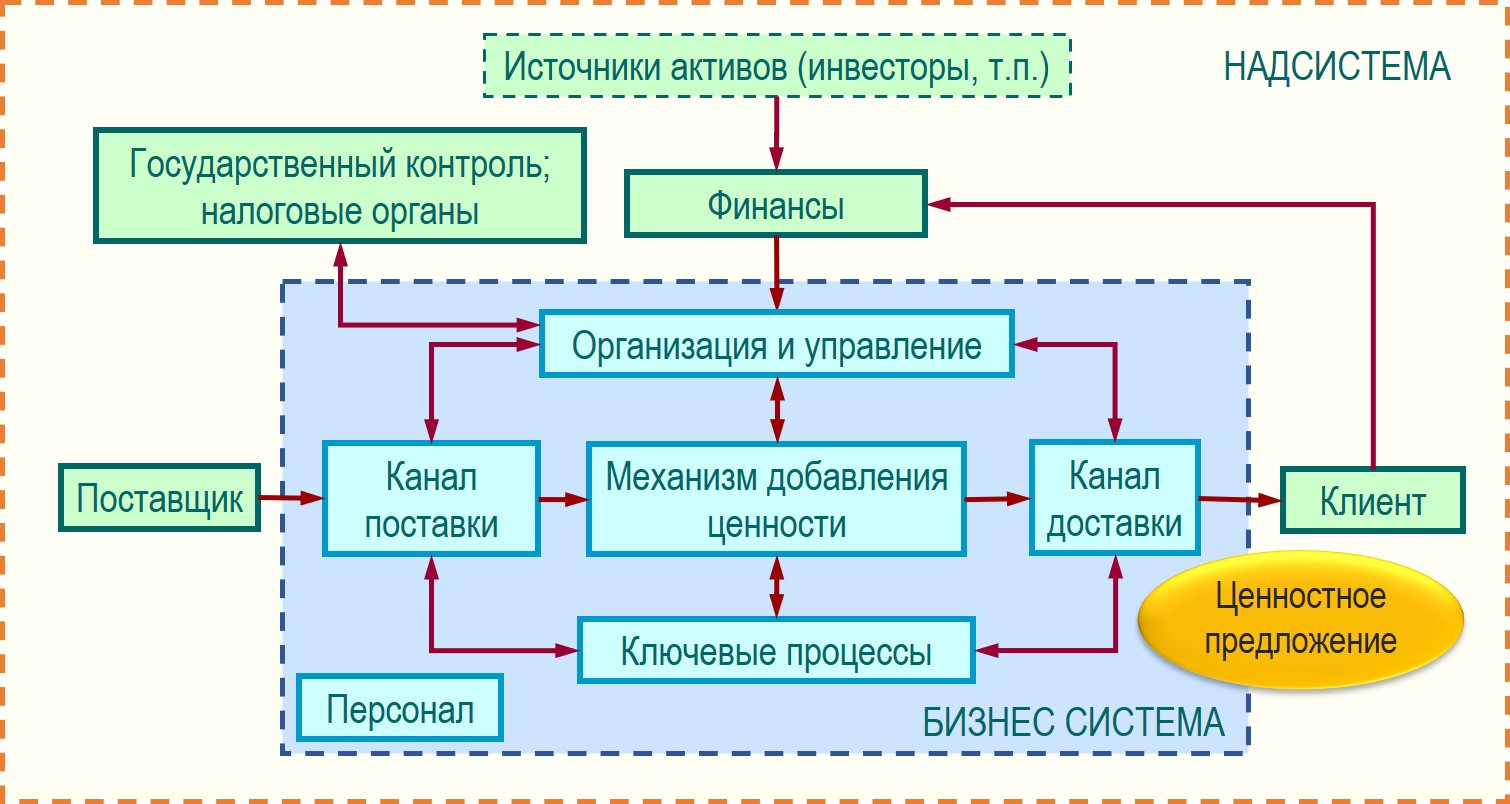
\includegraphics[width=.8\textwidth]{figures/fig.1.jpg}\\
  \textbf{Fig. 1.} Minimal viable business system.
\end{center}

As can be seen from the diagram in Fig. 1, for a business system to be
minimally viable, it must contain a supply engine, an added value creation
engine, and a delivery engine supplying value to the market. In addition, the
viability of the system is supported by business processes and management
functions (goal setting and control of their implementation), carriers of
these functions is the personnel of the company, in particular managers.
\textbf{In business systems, people are the most significant subsystems and
  supersystems}. The problem is that a person is a system with a high degree
of uncertainty (low probability of predictability of behavior), and therefore,
the same parameter of value at the input to the system can give a large spread
of output values depending on the specific state of the system element, and it
is often possible to observe a result that is very far from forecast.

Since a sustainable development of a business system is a primary goal, the
functions of setting tasks and monitoring their implementation requires a
clear vision from the manager [13], such that in business systems arise many
inventive situations, the resolution of which can clarify the vision of the
manager. It’s known that with many inventive tasks, a manager is not coping
due to the lack of a standard solution. In modern management it is estimated
that more than 90\% of managerial decisions are standardized [10], [23], but
remaining unsolved tasks may reduce the effectiveness of business systems, and
may remain unresolved for years, as practice shows. The author faced similar
tasks in the field of document management, staff recruitment and training,
marketing and sales, in the area of CRM systems ... The situation is
aggravated by the fact that it is not always easy to find and adapt decisions
from generally accepted practices -- OMT often need to be closed pretty
quickly.

Until these “white spots” can be overcome and clarity appears about their
design in the mind of the manager, the function of setting tasks for execution
and controlling them cannot be fully implemented. The business system is in
constant movement, therefore such “white spots“ in the activities of modern
managers arise with enviable frequency, and time to overcome them less and
less is spent from year to year. Similar tasks are called in this paper
\emph{organisational-managerial tasks} (OMT). They have good potential for
applying TRIZ tools and approaches.

Since the purpose of this work is to study the features of the application of
TRIZ to the class of tasks set in business systems there should be given
attention to the definition of OMT.

The author believes that in solving this class of problems it is worth to
distinguish three forms of activity that form the basis of management [41]:
\begin{itemize}[noitemsep]
\item organisation;
\item leadership;
\item management.
\end{itemize}
\emph{Organisation} is the process of forming supersystems and / or subsystems
of various level in business systems: associations, organisations,
departments, workplaces finally.  Organisation is the formation of the
structure, that is, of the elements and their interconnections.

\emph{Leadership} (from words to lead, lead by hands) is the setting of tasks
to performers and monitoring their implementation.

\emph{Management} is a change in the activities of performers. That is, when
the structure is organized, all tasks are distributed (including tasks for
feedback), but we are not satisfied with the efficency of the performers, we
are trying to change their activity in the direction of improvement, that is,
we begin to manage their activity.

All three of these activities form what can ultimately be called «Activities
in business systems». Therefore, I propose to call such a class of tasks
«organisational-managerial». \emph{Of course, from the standpoint of using
  TRIZ, we are only interested in inventive situations that arise when solving
  OMT.}  Further, using the term OMT, the presence of an inventive situation
will be implied.

However, before using TRIZ tools, an inventive situation should be previously
analyzed. Similar analysis in OMT has differences from pre-processing tasks in
technical systems, primarily because an element of the system is a human --
\emph{a complexly organized element that has its own goals}. Moreover, the
processes going on in such systems are often quite confuse, contain a lot of
interrelations which are hardly to grasp and dynamically changing and require
a special approach to their identification and description.

Below we discuss approaches used in both TRIZ and management consulting that
can be (and are) used for describing OMT and compare them with the method
proposed by the author of a description of an inventive situation in OMT.

\section[The SMART method]{Application of the SMART method to formalize
  organisational management tasks}

SMART [14] (the extended formula “SMARTER” is also used) is a mnemonic
abbreviation for the principle of setting goals. This model is today the basic
standard when setting tasks to subordinates, we can say that this is the main
international standard in this field. According to SMART, the task should be
specific, measurable, attainable, relevant, correlated with a specific period
(time-bounded). Perhaps this is the most world-famous way of formalizing OMT.
Examples of tasks set in accordance with the SMART model:
\begin{itemize}\it
\item [1)] 10\% of the employees are stably late for work for 5-10 minutes,
  another 3\% of the team are late for more than 15 minutes. As «stable delay»
  delays more than 5 times a month are considered. It is required to lower
  maximum stable lateness of employees up to 3, lateness of 15 minutes and
  above have completely to be excluded.
\item[2)] It is required to increase sales of the company's product
  (biologically active supplements from natural raw materials) by 20\% until
  December 31, 2017. Growth through expansion of territories is unacceptable,
  an increase should occur in existing territories.  Allowed increase in
  marketing budget -- 10\%.
\end{itemize}

This method of formalizing OMT is much better than the absence of any scheme,
however, it is easy to notice that such a statement of the problem is good for
execution in case the performers have all necessary resources to complete the
given task and if the performers know ways to accomplish it (they know how to
apply these resources to achieve the given goal). However, such a model is
completely insufficient for formalization of the task in order to find the
most effective conceptual solutions if there is no standard solution to the
problem. Consequently, the SMART model does not open up the possibility of
applying TRIZ methods, and therefore, it cannot be considered as a method of
preliminary formalization of the inventive situation.  In fact, the use of the
SMART model does not allow the solver to switch from the inventive situation
to a task (more precisely, to a system of tasks) suitable for further
processing using TRIZ tools. \textbf{In the opinion of the author, what makes
  the use of TRIZ in the first place difficult for the solution of OMT is the
  lack of reliable and relatively simple tools, allowing to move from an
  inventive situation to a system of tasks in the field of business systems}.

The SMART model, though, makes important refinements to the understanding of
the inventive situation, but does not solve the problem of preparing an
inventive situation in OMT for further processing by TRIZ methods. Currently,
the SMART method is a generally accepted method of goal setting all over the
world, mastery of the SMART method is considered as one of the most important
competencies of a modern manager, as almost indispensable management basics.
However, to formalize the inventive situation in OMT, this generally accepted
method does not give the required result -- it does not help to derive a
system of tasks from an inventive situation, which can subsequently be
processed with TRIZ tools.

There is also another opinion. For example, a number of TRIZ specialists are
convinced that if there are no standard methods or not enough resources to
solve the given problem, then any TRIZ specialist will formulate a
contradiction using standard formulas.  The author strongly disagrees with
this argument, since before a contradiction can be formulated according to
standard formulas, for a successful solution of the OMT it is required to
describe a model of a working business system (MWS) [15] and set up a system
of particular tasks to its elements (subsystems and supersystems). Otherwise,
we get a contradiction that is of extremely general nature, and therefore,
there is a high risk of getting trivial decisions as output. The author
recommends to formulate contradictions to each of the particular tasks posed
after the analysis of the MWS. Otherwise, the solver risks that the obtained
solutions are to «narrow», and as a result, a situation is possible when the
solver will not finally reach the goal [10], [11].

It is worth noting that the tree of contradictions also cannot be used on this
stage, since at the stage of formulating the OMT the set of contradictions is
not yet visible -- see the example at the end of the section (the problem of
implementation a new sales system in the company).

\textbf{Conclusion: the SMART method helps to specify the task to be
  performed, but cannot be used as a tool for initial processing of an
  inventive situation.}

\section{Description of business processes}

Description of business processes [34] is another method that is actively used
in an consulting environment for preliminary processing of an inventive
situation.  It is usually resorted to the description of business processes if
the solver believes that an organized social system does not function
rationally, which means, unlike the previous method of tasks setting, has a
narrower scope. As a rule, this tool is used to analyze the inventive
situation in order to increase the efficiency of standard, well-established
processes in organized social systems.

The technology for describing business processes in the worldwide practice is
standardized and described by generally accepted \emph{notations}, e.g. IDEF0,
BPMN and others [34]. In TRIZ, a similar method is also actively used in the
form of \emph{flow analysis}. And although the descriptions of business
processes and the flow analysis are not quite the same thing [11] (flow
analysis describes the transfer of matter, energy or information, has sources,
consumers and a flow path, whereas the description of a business process
focuses on a list of operations performed by the process owner and process
members), these methods have a lot in common.

An example of a business process description:

\addpicture{Fig. 2. An example of a description of a business process.}

In fig. 2 an example of a description of a business process of decision-making
by a bank on a client’s loan application is shown using BPMN notation. As can
be seen from fig. 2, a similar method is well suited for preliminary analytics
of only one class of OMT: optimization of regularly recurring operations in
various parts of the organized social system.  But if the task is connected
not only with established processes, what to do in this case? After all,
business processes are only one aspect of the development of organized social
systems, there are also other levels -- making strategic decisions, developing
new directions of activities, relationships of process participants and other
tasks.

\textbf{Conclusion: the tool is very useful in solving a particular class of
  OMT but does not possess the required versatility and is suitable
  exclusively for optimization of regularly ongoing processes, and therefore,
  as a single tool for preliminary processing of an inventive situation for
  solving OMT cannot be recommended.}

\section{System Operator}
Let's consider the «classic» TRIZ tools that is claimed to be used for primary
analysis of an inventive situation in OMT.

There are known cases, where TRIZ practitioners use the system operator for
this purpose [25]. The author also applies the system operator to solve
problems in business systems. One example of the application of the system
operator to solve an OMT is shown in Appendix 2.  With the help of the system
operator it is possible to see the dynamics of development of a system and
predict its structure in the future, and also to consider the structure of the
functioning system -- to describe supersystems and subsystems of the given
system (... sub-subsystems, subsystems, system, supersystems,
super-supersystems ...).

Indeed, the system operator has a significant drawback -- it is looking at the
development of the system through the composition of its elements, but does
not take into account the layers of the system and the relations between its
elements. This, of course, cardinally limits the capabilities of this tool for
a descriptions of organized social systems. In addition, the structure of a
working system is taken only element-wise, in contrast to the schematization
that looks through the layers, groups, relations, processes and functions. And
if the supersystems are on completely different management layers, what to do
in this case? How to set specific tasks for effectiveness of management of
system elements?  The system operator does not reflect management phenomena
(fig. 3).

The advantages of the system operator include its versatility and adjustable
level of detail of system elements, as well as the ability to trace the
evolution of the system, its subsystems and supersystems, what determines the
prognostic value of the tool.

The downside is the impossibility of an adjustable decomposition of elements
of the supersystem, the impossibility of drawing relationships between
elements of the system and the supersystem (the structure is taken as if in
isolation, without indicating the connections between the elements of the
system), as well as the impossibility of demonstrating in the model the
schemes of control, which is a critically nessecary moment when studying the
inventive situation with the aim to solve OMT.

\addpicture{Fig. 3. The structure of the system operator.}

Nevertheless, the author considers the system operator a perfectly applicable
tool to solve OMT, but not for the purpose of preliminary analysis of the
inventive situation, but \textbf{in order to study the system in the context
  of its evolution} [11], which is important for a number of
\textbf{strategic} tasks, where situational interactions of elements of the
system should not be taken into account.

\textbf{In contrast to the specific inventive situation posed by the customer
  in an organized social system, tasks that should be studied using the system
  operator, are usually general and strategic in nature (see Appendix 2).}

\section{Structural Analysis and Functional Modeling}
These types of analysis applied in a FVA [19], most accurately describe the
inventive situation when solving OMT, since they show the composition of the
system, elements of the supersystem, the relationship between the elements of
the system, functions, and modern versions of FVA allow you to extract groups
of elements and even to take into account the processes within the system
[17]. An example of a functional scheme is shown in fig. 4:

\addpicture{Fig. 4. Simplified functional scheme of a construction worker's
  helmet (in red harmful functions are shown).}

It is this approach that makes it possible to conduct a preliminary analysis
of the inventive situation with the aim of setting particular tasks, which
subsequently can be solved using TRIZ tools. However, functional modelling has
all the same key defects as any method developed for analysis of technical
systems: the method does not take into account the management context between
elements of the system. Moreover, a part of the elements of a working system
are good modifiable objects of the material world, and some are subjects, that
is, people, performing defined functions, but with their own goals,
dynamically changing emotions, patterns of behavior, etc., that is, objects
with behavior which is hard to predict.  The description of such objects
requires a special language in order to develop solutions that can later be
replicated.

When solving OMT, it is impossible to ignore such phenomena, since people in
organized social systems are essential (and often the most important) elements
of the system.

\textbf{Conclusion: The author believes that functional analysis has great
  potential for solving OMT -- in the author’s book [11] an example of a
  solution of a similar problem is explained in detail --, but this tool is
  more likely applicable to a certain class of OMT related to the optimization
  of organized social systems and their subsystems [39] and is not very
  convenient for preliminary analysis of inventive situations arising in such
  systems, since it does not take into account the specifics of a description
  of people as subsystems of a social system, nor does it take into account
  the dynamically changing driving influence of the elements of the system to
  each other in the context of the inventive situation under consideraton
  (i.e., it does not take into account the peculiarities of «soft» systems).}

\section[Schematization at MMK]{Schematization developed at the Moscow
  Methodological a circle (MMK) under the leadership of G.P. Shchedrovitsky
  and its application for preliminary inventive analysis of inventive
  situations}

This method was formed in the Moscow Methodological Circle under the
leadership of G.P. Schedrovitsky [10] in order to organize the thought
activity (\foreignlanguage{russian}{мыследеятельность}) of a group of
professionals who discuss problematic situations in the field of organisation
and management. The meaning of this tool was to gradually put on the «Map» the
elements of the system that are significant for the task being solved and
relations between them, that is, get a tool for the manager, similar to the
main tools of military strategists -- a map, the details of which are
appearing gradually, in the course of the thought activity of the officers
planning the military operation. The author considers such workout to be an
excellent alternative to the methods described above from the point of view of
formalizing the inventive situation, but getting a synthesis of schematization
and TRIZ in its purest form was not so easy.

Essentially, schematization is a visualization of an inventive situation
worked out in accordance with the \textbf{system categories} and understanding
the functionality of the system [10]. It is this tool that the author
considers optimal for a primary analysis of an inventive situation when
solving OMT. It should be noted that the author had to restore the following
categories of schematization on his own, based on a detailed study of the
works of G.P. Shchedrovitsky, as currently schematization is greatly
simplified and many SMD methodologists are building schemes without taking
into account the categories of systems described below.  Some of them even
generally simplified schematization to scribing [35].

Therefore, the author had to restore the principles of schematization from the
work of G.P. Schedrovitsky, and then develop on his own methods for setting
tasks based on the results of a schematization of the inventive situation in
OMT.

Based on the analysis of the works of G.P. Schedrovitsky the following
categories of schematization can be distinguished:
\begin{itemize}[noitemsep]
\item[1.] MWS (model of a working system -- frame);
\item[2.] Layers;
\item[3.] Groups;
\item[4.] Relations;
\item[5.] Functions;
\item[6.] Processes;
\item[7.] Generalized Objects;
\item[8.] Fillings.
\end{itemize}

A caveat is required: the category \textbf{«system frame»} in the
terminological apparatus of G.P. Shchedrovitsky can be replaced by the
category \textbf{«model of a working system»} developed by Nikolai Shpakovsky
[15].

Since the author spent a significant part of his work in departments of
marketing and sales of international corporations and is the author of a
three-volume book «The era of smart sales ...», where he summarized the
experience gained and described his methodological basics in this area, and
currently leads a significant part of projects in the field of marketing and
sales in the B2B market [27], many examples of OMT the author takes from these
areas. Of course, this does not mean that OMT are restricted to the field of
marketing and sales. The converse is true: problems from marketing and sales
are a special kind of OMT.

\subsection{The model of a working system (MWS) is determined in two stages:}

\subsubsection*{1. Isolation of the kernel.}

The inventive situation presented by the stakeholder indicates that there is
resistance of managers who do not accept the new sales system, implemented at
the enterprise. It’s known that before that, managers didn’t work chaotic,
their work was determined by a different sales technology supported at the
enterprise, to which they adopted. After conducting these simple arguments, we
identified the structural core, which can be represented as part of a scheme
(Fig. 5):

\addpicture{Fig. 5. The core of the problem, presented in the form of a
  scheme.}

In fig. 5 we see the main stakeholder in the task -- the «resisting» managers
themselves, to what they resist -- the complex sales system being implemented
-- and the existing sales system, to which they adopted during time.  The two
sales systems conflict with each other (this is a logical conflict), in this
case -- differ in content and requirements, as shown by a dashed arrow, in
addition, managers also conflict with the newly introduced sales system, as it
requires them to restructure their work, which causes dissatisfaction with the
salespeople.  The new system is promoted by the head of the sales department,
so between the head of the sales department and the managers, we also observe
a conflict of interest. Further on the diagram we show also this connection.
\textbf{The core of the scheme always represents the minimal scheme of
  conflict given by the inventive situation.}

\subsubsection*{2. Definition of connections from the core of the task to the
  supersystem and the final definition of the MWS (frame).}

To whom the managers express their dissatisfaction, who perceives their
resistance? In the course of communication with the client, it turns out that
first of all -- to the head of the sales department (in the diagram in fig. 6
he is designated as ROP). And maybe also to customers, which is inacceptable
to the company. In any case, customers should be introduced in the scheme,
since they are ultimately affected by the internal changes in the sales
department.

Why was the sales system created? To increase conversion rates, efficiency of
work with the client, and as a result -- to sign more transactions on large
amounts without hiring additional sales staff. What else «hurts» the sales
system? The CRM system (Customer Relationship Management [16]) implemented in
the company. The new sales system requires major changes to the work with the
main software in the sales department -- the CRM system. Therefore, the scheme
depicts a conflict of the new sales system with the existing CRM system, to
which specialists of the sales department adopted. The problem is not that the
installed system does not have certain options, this is a secondary problem, a
smaller one than the one we trying to formalize. The problem is that the
«relationship» of the sales staff changed with the new requirements of the CRM
system.

In addition, the work of the sales department relates to activities of other
company services -- production, warehouse, logistics, accounting ... This is
important, but at the stage of setting the task it is too early to engage in a
deeper detailing of these processes; therefore, we denote these «touch points»
of the sales department with other company services as «cross-business
processes», which can also be transformed under the influence of the new sales
model. So we got a formed \textbf{model of a working system} consisting of:
sales staff, head of sales, the existing sales system, the new sales system
that is replacing it, the target client groups, CRM systems and cross-business
processes:

\addpicture{Fig. 6. A model of a working system, presented in the form of
  a diagram. Abbr.: ROP -- Head of Sales Department.}

\subsection{The concept of a layer in a scheme.}

A layer in a scheme symbolizes that an element of the system element or a
group of elements, placed on a higher layer controls an element or group of
elements, located on the lower layers in the context of the task (i.e. a layer
is a graphical representation of the fact of controlling the activities of one
element in relation to another).  And although the system is in most cases
defined as a set of interconnected elements, it is obvious that the elements
can have different hierarchical positions in the system to be studied, that
is, there is a hierarchy of control between the elements from the viewpoint of
a \emph{defined action} considered in the context of the problem to be solved.
The concept of a layer allows to consider the elements of the system, taking
into account their dynamically changing hierarchy, where the hierarchy is
determined on the basis of understanding which element is governing, and which
element carries out the «orders» of the more «senior» elements of the system,
and not in general, but only in the context of this specific activity related
to the considered OMT.

It is worth noting that the concept of a layer does not replace the concepts
of a sub-sub-system, subsystem, system, supersystem, etc., so layers are not
at all the same as what we depict in the system operator.  \emph{If
  subsystems, supersystems, etc. are fairly rigidly fixed, the layers are
  constantly changing in the context of the activities of the elements
  depicted in the scheme.}

That is, as an important concept for the analysis of business systems, the
author suggests to use schematization with the allocation of «layers»,
explaining this with the basic properties of organisational-managerial systems
built on a \emph{dynamically changing hierarchy of governance in the context
  of the studied activity of elements of the system}.

It is important to note that subsystems are subsets of the system, the system
itself is a subset of the supersystem. As you know, subsets have the property
of similarity to the sets of which they are a part. In other words, a
subsystem is a set of elements that make up the system, broken down by some
criteria into subsets [45].

For example, a subset of the decision center [16] in an organisation is a
seller of the company -- a potential supplier of the product, since the seller
is a subset from a decision-making perspective (he makes a decision based on
information transmitted to the seller, but not only. In the process of
decision the decision center is influenced also by other subsets). But which
element rules which activities of other elements? This is a big question. The
answer can be given only in the context of the task.  Suppose, in the process
of implementing his functions, the manager conducts research on customer
needs, on the basis of which he subsequently prepares a commercial proposal.
Which element of activity controls which? \emph{Of course, the client controls
  the further actions of the seller based on the information provided about
  his needs}. Moreover, if we consider a different situation, where the needs
of the customer is a product, then the layers will change again, that is, the
seller through questions will manage the activities of the decision center. At
the same time, the subsystem and supersystem remained at their places, only
layers change!  Another example. The seller forms a picture of the world of
the customer, creating value in his offer. Which element is now driving the
activity of which? Now the seller drives the activities of the client from a
position of acceptance of the solutions.  The subsystem governs activities of
the supersystem in this context.  Please note: subsystem and supersystem did
not change places, but layers -- changed!

This is the most important understanding from the point of view of finding a
solution to a problem in an organisational-managerial context, therefore, the
concept of a layer is not a substitute for the concepts of supersystem and
subsystem.

\textbf{Rule for representing layers in a diagram:} If any elements of the
system are depicted in the diagram higher than the others, then the solver
ranks them in the upper layer, i.e. in the context of this inventive situation
considers them as controlling elements. The main thing is to always remember
the rule: layers may vary depending on the contemplated inventive situation.

In fig. 6 layers are clearly visible in the context of the task: Cross-cutting
business processes have largely determined the configuration of an existing
CRM system. The CRM system, which was configured based on the requirements of
the existing sales system, at the moment is a deterrent to the implementation
of the new sales system, as it is reliably connected with end-to-end business
processes in the company, which implies the use of its reports by a number of
related units. It does not support the functions required for the new sales
system, but the transition to another CRM system, although it will provide the
necessary functions for the introduction of the new sales system, is highly
likely to give rise to similar conflicts at the border of the sales department
with other divisions of the company. From here it’s easy to conclude that the
sales staff are on the next layer -- they are «controlled» by the existing
business processes in the company and the «adapted» to them CRM system that
supports the current sales system, which, in its turn, does not suit the head
of the sales department and the best employees, since it does not support
effective work with clients in recent conditions on a highly competitive
market.

It is not hard to notice that the schematic representation of the MWS taking
into account the layers makes a lot of important refinements in understanding
the inventive situation. The analysis of the schemes shows that there are at
least several contradictions hidden in the problem (\emph{of course, such a
  representation of an inventive situation requires the solver to develop
  schematization skills, so in the process of constructing a scheme a
  bidirectional thought process is going on: the scheme is built in the
  process of analyzing the layers, but on the other hand, layers «appear» in
  the process of constructing the scheme. Therefore, in practice, the scheme
  of the MWS is usually redrawn several times, until full clarity is
  established in the description of the inventive situation between the
  problem owner and the solver}).

To this point, the author received the remark that since a scheme is rarely
created in one passage, this approach strongly resembles the method of trial
and error. The author does not consider the method of trial and error and
iterative approach as identical concepts, as during several iterations the
scheme is refined, and is not newly created in a random manner.  The solver
also clarifies the definitions when formulating a technical contradition or an
IFR.  It is far from always possible to get the final wording in the first
attempt. The same happens when applying schematization.

\subsection{Groups of elements of the MWS (groups)}

A group is a combination of elements of a system to fulfill a specific
function.  If the group is taken as a separate system, then we can talk about
the MUF (main useful function) of the group. \emph{The author believes that
  instead of the term «group», introduced by G.P. Shchedrovitsky, it is
  completely appropriate to use the TRIZ terms -- system, subsystem,
  sub-subsystem ...}. Usually, if solving a problem requires a more general
consideration of the elements of the system, or a more detailed one (in the
course of work on the task such transitions are assumed and become apparent in
the communication process between the solver and the problem provider), it is
convenient to give on the scheme the required detailing of the elements and
their relationships for deeper analysis, but in the moment when more
superficial analysis is required, combine such elements (sub-subsystems) into
groups (subsystems) and emphasize the general function of the group. In
practical applications of schematization for the analysis of an inventive
situation, such a division may be very important, for example, for the task of
increasing the efficiency of a department (in this case, the sales department)
the following scheme was developed for the analysis of an inventive situation:

\addpicture{Fig. 7. Scheme of the sales department with the allocation of
  layers and groups. Abbr .: KAM -- key account manager, lead -- potential
  client who in one way or another responded to marketing communication.}

The groups in the diagram are:
\begin{itemize}[noitemsep]
\item marketing department; 
\item sales department; 
\item customers.
\end{itemize}
For example, why did the company create a marketing department? To prepare and
conduct marketing promotions? To study the market? For advertising campaigns?
For marketing analytics? To carry out public relations (PR)? Marketing should
carry out all these functions, but they are not the main ones. They are
auxiliary ones. All these functions are needed in order to promote your
product on the market. So the MUF of the group of marketing (department) is
the promotion of the company's product on the market by influencing target
client groups (again groups, only now they are combined by functional features
of consumption). The MUF of the group (department) sales is the same, but with
some differences -- promoting a company's product on the market by personal
impact on the client. The difference between them is essential in the way how
they impact on the target audience.

Groups can be not only departments and divisions. It can be project groups or,
for example, groups of employees united by some social characteristic or, say,
the time of work in the company. It all depends on the condition of the task.
Only one very important rule should be remembered. Any group has its own MUF
that is significant for the problem to be solved. An arbitrary division of
elements into groups within the frame of a working system is unacceptable, as
this complicates the task, burdens it with unnecessary information.  The
question arises: is it worth to introduce this concept or to stick to the
notion of a subsystem, traditionally used in TRIZ? Is it possible to use the
concept of «aggregation of elements» instead of «groups» also known in TRIZ?
At this stage the author proposes to leave this debatable question open.

\paragraph{Functions.}
Functional language is perfectly developed in TRIZ and, perhaps, is the main
language used in the analysis and description of a system: first of all, with
the use of FVA. Therefore in this work, a detailed description of the concept
of a «function» is not required.

\paragraph{Processes and communications.}
These are the most important categories of schematization.

A \emph{process} is the development of a phenomenon in time. In this
definition the key word is «phenomenon».

\emph{Relationships} are a designation on the scheme showing that in the
context of the task it is important for us that element A affects element B,
but what processes are going on is not important for us.

Since the scheme in fig. 7 is functional, processes are not indicated on it,
but functions are shown as arrows. But when creating a functional scheme it is
not managed to get a working model, that is, when analyzing the scheme,
disruptions and promising trajectories of the problem solution became not
visible, then you should embark into processes.

Interestingly, in TRIZ this problem of the process level has already been
discussed, for example, in relation to \emph{advanced functional analysis}
developed by Naum and Oleg Feigenson [17] when, as a result of the FVA not
one, but several functional models are built, each for a specific state of the
system due to the processes occurring in the system.

Here we can clearly see the fact that in most problems the solver may remain
at the functional level (then on the scheme only functions and relations are
present), but there are situations when the system has to be considered in
various states depending on the processes occurring in it. Similarly, when
conducting schematization of an inventive situation, there are situations when
the scheme requires to indicate also the processes going on between the
elements of the system. Understanding the difference between processes and
relationships is very important for a qualitative schematization of the
inventive situation when solving OMT.

You can see an example of such a scheme in the diagram below:

\addpicture{Fig. 8. The scheme of analysis of the inventive situation of the
  problem of increasing the effectiveness of the mentoring process.}

In the diagram shown in fig. 8, the modelling of the mentoring process is
visible, that is organized in the sales department. The processes indicated by
arrows are considered in detail that go on when planning a strategy for
concluding a deal, the student’s work in «field conditions» and the processes
that occur during the organisation of feedback from the student to the mentor.
In addition, the task involves in-depth study of the processes taking place in
the period of supervision by the mentor of the development of the student's
skill in using the tool, which the latter should develop on the instructions
of the mentor.

\textbf{Up today, the author does not have data on the existence of a
  methodology to clearly determine during schematization whether a transition
  to a process level is required, or it is sufficient to remain on the level
  of a scheme containing only the necessary elements, their functions and
  relationships.} The practical recommendation is as follows: first we build a
scheme describing the inventive situation at the level of relationships and
functions, and then, if the data is clearly not enough for further processing
by TRIZ tools, we begin to delve into the consideration of processes between
system elements, for which flow analysis or analysis of business processes
using standardized notations is applied [34].

Introducing processes in the scheme leads to inevitable complications of the
scheme, describing the inventive situation, therefore, when conducting
schematization one should be guided by the principle of appropriateness and
introduce processes only if there is a need for their detailed study (see the
case of the introduction of a new sales systems below, appendix 5).

\paragraph{Generalized objects and filling.}

Let's move on to the concept of «generalized object» and «filling». In the
opinion of the author, from the categories developed by G.P. Shchedrovitsky,
these concepts are one of the keys in terms of applying system analysis to
inventive situations arising in the field of organisation and management.
These categories applied to schematization are responsible for scaling the
received solution.  \textbf{Scaling is the most important characteristics of
  the obtained solution in the organisational-managerial sphere.}

When conducting schematization from the position of the categories
«generalized object» and «filling», not only the likelihood of a scalable
solution sharply increases, but also its stability, that is, the ability to
withstand environmental disturbances. In fact, at the stage of schematizing
the inventive situation, the foundation is laid of the quality of the future
solution.

A \emph{generalized object} is a vacant unit, a kind of «shell» of an element,
which specifies the requirements for that element.

Generalized objects have \emph{properties that pose requirements on their
  filling}. For example, generalized object «head», generalised object
«teacher», etc.

Generalized objects are linked to other generalized objects in the structure,
but in order for the system to function, the generalized objects must be
filled.  Someone must be a miller, a supervisor, a driver -- e.g., a computer
program or a person (see Figure 1 -- it is indicated that a person is a
subsystem or a supersystem of an organised social system (using the business
as an example), although if we look at it in more detail, the subsystem or
supersystem would not be a person as such, but a generalized object, which
should have the appropriate filling). A \textbf{filling} is the system that
fills the generalized object according to the requirements of that entity,
e.g. a person with relevant competences or, for example, a computer program
with certain characteristics corresponding to the requirements of the
generalized entity.

In the technology of G.P. Shchedrovitsky's the requirements of generalized
objects are called \emph{properties-functions}, and the properties of filling
\emph{attributive properties}.  (In G. P. Shchedrovitsky's texts generalized
objects are named «places», but the author believes that such a name is more
likely to cause confusion). So in OMT there arises a special class of tasks --
tasks that \emph{coordinate} requirements of generalized objects
(properties-functions) and filling properties (attributive properties).

When solving OMT, the solver must understand on which layer should he solve
the task.  If the task is solved in the space of the organisation or its units
(department, department, site), it is important to try to find a solution on
the level of generalized objects, which will determine the further scaling of
the obtained solution.  If the task is set at the level of a specific filling,
then the solver should warn the customer that the solution is likely to be
special for this case and scaling of the obtained solution will be difficult
(if at all possible).

Generalized objects can be represented as subjects (this is a generalized
object that takes people as filling), and objects (taking a computer program,
any document, robot, etc. as filling, see fig. 9).

Some notation used in the diagrams :

\addpicture{Fig. 9. Some designations used in the scheme of the inventive
  situation.} 

\section{Setting objectives based on the results of schematization}

\textbf{Two versions for further analysis after schematization have to be
  distinguished:} 

\paragraph{Option 1. Work with existing disruptions.}
We find \emph{disruptions}, i.e.  discrepancies between «how it should be» and
what is currently depicted on the scheme. Particular tasks can be set from
disruptions (\textbf{see appendix 1}).

Next, we highlight a list of harmful effects (HE). Working with harmful
effects is well developed in TRIZ, most often for this purpose cause-effect
analysis is applied. Therefore, according to the results of schematization of
an inventive situation, we can advance in a variety of ways:

We get a list of HE and conduct a cause-effect analysis. This approach can be
applied if all NE in the diagram are obvious;

We identify the disruptions in the diagram and set the task to eliminate them.
To the received tasks, you can apply the primary processing mechanisms of a
task, long and successfully used in TRIZ -- flow analysis, functional
analysis, cause-effect analysis, benchmarking ... [18]. There are many
variations, we move depending on the context. No one forbids applying
schematization to clarify in detail the structure of the disruption, if the
obtained task is a new inventive situation with many unknowns [11];

Highlight technical contradictions and continue to work with them
(\emph{technical contradiction: a situation that arises when trying to solve
  an inventive task by improving a specific feature (parameter) of the system,
  which leads to unacceptable degradation of another feature (parameter) of
  the same system} [42]). In that case decisive TRIZ mechanisms come into
operation.

\paragraph{Option 2. Choosing a promising roadmap and setting private tasks.}
This was the path we took, solving the problem of a multiple increase in sales
of construction equipment in the channel «road construction» (fig. 10). The
problem was that over the past three years, the company's product margin has
been halved, and sales were steadily falling. Marginality is known to add up
from costs structure and market value. We decided to start from the second and
analyzed the structure of the construction equipment market (fig. 10 gives an
example of a raw analysis of the situation, but in order to understand that
the current business strategy of the company has been chosen incorrectly,
schematization without finegraned detail turned out to be sufficient):

\addpicture{Fig. 10. Preliminary «raw» scheme of the design of the
  construction equipment market in the Southern Ural.}

To come to the choice of a promising road map, we plotted budget allocation
for road construction and sorted out the hierarchy of this distribution -- so
the layers in this diagram were grouped by regions (groups). Further,
understanding the price segmentation of construction equipment, it turned out
to be easy to compare these two parameters with the practice at the client
side, and then highlight two points on the scheme -- \emph{layers} that the
company is working with now and the layer as much as possible close to the
consumer, capable of acquiring the technics of this segment based on the data
plotted on the scheme and its typical needs. \emph{So a promising roadmap was
  decided, which was significantly different from the existing company’s
  market strategy}. To implement the resulting roadmap it was required to pose
a number of tasks and resolve the contradictions that arose.

At first glance, it may seem that this scenario is similar to the construction
of a functional model during FVA, as both the scheme and the functional model
describe the structure of the system. However, the \textbf{scheme refines also
  the layers, showing the dynamical hierarchy of control, additionally
  allowing to model the depth of interaction between system elements, by
  introducing a chain of concepts of relation-function-process, and reveals
  the composition of the subsystems, if this is necessary from the position of
  the task being solved} (groups or aggregation of elements). This includes
the ability to select groups passing through layers «diagonally», for example,
if by the condition of the task there is a need to analyze the work of project
teams taking into account employees in two or more roles (for example, a
member of the project team is a financial officer). \textbf{When conducting
  schematization, the solver has the ability to distinguish between the
  filling property and the requirements of generalized objects, which is
  critical important from the point of view of scalability of the resulting
  solution} (another example of an inventive situation is depicted in the
diagram in fig. 11).

\addpicture{Fig. 11. The scheme of selection of employees according to the
  competency model.}

Fig. 11 shows a scheme compiled by the author to describe an inventive
situation that arose during the selection of employees for certain positions
taking into account changes in the requirements of generalized objects during
the evolution of the organisation according to the model of I. Adizes (fig. 11
shows the so-called PAEI code (P -- production of results, A --
administration, E -- entrepreneurial function and I -- integration. PAE is
more about generalized objects, I is more about filling). The PAEI code is
shown in fig. 11 as a function of the requirements of generalized objects and
properties of their filling.  In the scheme also significant roles of process
participants are visible which are located on three layers and elements of the
recruitment systems related to generalized objects (competency model) and
filling (competency assessment, personality type and ability assessment).

Therefore, despite a certain similarity with the functional model, the scheme
is a slightly different tool. Its \textbf{main purpose is to isolate the
  system of tasks from the primary inventive situation}. The author suggests
using schematization to formalize the inventive situation when solving OMT.
Schematization should be applied immediately after clarification of the core
of the problem and the goals of the solver before using the usual TRIZ tools.

\section{The fundamental difference between schematization and functional
  modelling} 

\paragraph{Layer Selection.}
The functional model used in the FVA does not imply building a hierarchical
scheme with the allocation of layers, where the subject of management is in a
higher layer in comparison with the controlled object. A similar hierarchy of
elements in the scheme is very important for the analysis of an inventive
situation in OMT (the very concept of organisational-\emph{managerial} tasks
requires a representations of system elements depending on the control hierarchy
in terms of allocated task).

\paragraph{Representation of a system element as a Generalized Object and
  Filling, }
clear realization whether we are solving the problem at the level of a
\emph{generalized object} or at the level of the \emph{filling}. The author
pointed out above that business systems are soft systems, as they include
human as the main subsystems.

\textbf{The author emphasizes once again that a simple tool transfer from
  technical to business systems is not possible. To handle an inventive
  situation in business systems requires specific tools that prepare a task to
  use «standard» TRIZ tools.}

\section{The algorithm for working with a scheme}

The algorithm for working with a scheme goes as follows:
\begin{itemize}
\item Based on the situational analysis that we carry out on the scheme, the
  most acceptable way of conducting further transformations is chosen, which
  is defined on a priority basis (road map of future moves).
\item As soon as the roadmap is selected, we immediately attaching it to the
  existing system see the secondary tasks in the form of directions or HE,
  which will appear in the system when implementing the selected roadmap.
\item If necessary, we analyze the selected tasks with tools of primary task
  processing adopted in TRIZ.
\item If necessary, we form technical contradictions.  Next for the solution
  of the selected contradictions we apply the known TRIZ tools.
\end{itemize}

\section[Applying schematization]{An example of the use of schematization for
  setting objectives for organisational and managerial task (the case is
  described in detail in Appendix 5):}

\textbf{Given is a system consisting of:} sales department of an industrial
enterprise, manufacturing tooling from heat-resistant steel, presented by the
head of sales, sales staff and the current sales system sales (fig. 12).

\textbf{The essence of the problem:} the head of sales (ROP) implements a new
sales system, having advantages over the previous one in terms of depth of
study of customers and, as a result, allowing to increase the average amount of
contracts and conversion, however, managers resist and are in no hurry to
leave the «retrackted tracks».

\textbf{Required:} to make managers use only the tools of the new sales system
in their activities (the task in the original formulation, that in the process
of analyzing the scheme turned out to be not quite the correct goal setting --
see the table).

Below, we compose a MWS, presented in the form of a scheme.  The process of
constructing a scheme for this task is described above (see explanations for
fig. 6):

\addpicture{Fig. 12. The scheme of the inventive situation in the problem of
  changing the sales system.}

The tasks set according to the scheme (fig. 12) using the categories of
schematization\footnote{In the original text displayed as table with 3
  columns.}:

%--- start table
\begin{itemize}
\item[1.] Interaction of the system (dotted line) with the elements of the
  supersystems
  \begin{itemize}
  \item[1.1.]  \emph{The CRM system}. The conflict arose largely due to the
    fact that the existing CRM system is not adapted to the requirements of
    the new sales system, which creates significant inconvenience
    \textbf{$\to$ Make the CRM system meet the requirements of the new sales
      system and supported it.}
  \item [1.2.] \emph{Cross-business processes}. The new sales system changes
    the cross-business processes, this has especially an impact on the
    collaboration with the design department and the production \textbf{$\to$
      Configure cross-business processes in such a way that the requirements
      of the new sales systems are provided.}
  \item [1.3.]  \emph{Customers}. The new sales system increases the time for
    a contact with the customer \textbf{$\to$ Increase the depth of the work
      with the customers without increasing the time expenses of the
      managers?}
  \end{itemize}
\item [2.] \textbf{Layers}
  \begin{itemize}
  \item [2.1.] The implemented sales system influences the actions of the
    managers, imposing on them specific requirements \textbf{$\to$ How to make
      the sales system requirements performed, but the managers have to spend
      as little effort as possible?}
  \item [2.2.] Managers are faced with the fact that for a number of clients
    the requirements of the new system are redundant, which does not increase,
    but rather reduces efficiency (\emph{from this point of view managers
      «control» the reaction of customers, hence the given distribution of the
      layers on the scheme}) \textbf{$\to$ Differentiate customers and
      introduce the new sales system only in relation to such client groups in
      which conversion increase and average weight of the transaction is
      expected when applying this system.}
  \end{itemize}
\item [3.] Communications. \emph{Partially analyzed in paragraphs 1 and 2,
  additionally:}
  \begin{itemize}
  \item [3.1.] A logical conflict between two systems, for example, the
    approach to identification of needs, the stages of the transaction are
    radically different. \textbf{$\to$ Compare the requirements of the
      existing and new systems, identify areas of similarities and cardinal
      discrepancies, disassemble into elementary steps of the area of cardinal
      differences, thereby simplifying the implementation} (such an approach
    to the problem allows the solver to rely on existing resources).
  \item [3.2.] Communication defects in the line head of sales -- managers
    \textbf{$\to$ Define metrics and reference points in the new sales system,
      which should provide feedback from the manager to the head. Simplify the
      data retrieval for the managers on reference points.}
  \item [3.3.] Establish a relationship CRM system -- head of sales $\to$
    Having solved the tasks 3.2, \textbf{bring the CRM system in accordance
      with the received solutions, incorporate accordingly changes in the
      schedules of the meetings, strengthen communication on reference points
      and reduce communication on less essential items.}
  \end{itemize}
\item [4.] Processes and functions
  \begin{itemize}
  \item [4.1.] \emph{The task appeared after setting the task 1.2:}
    \textbf{Conduct a detailed analysis of business processes between the
      sales department and the design department, as well as between the sales
      department and the production department} (compiling in advace a map of
    processes in BPMN notation). \textbf{Highlight the bottlenecks and set
      tasks to overcome them.}
  \item [4.2.]  \emph{After solving task 1.1}, \textbf{set the task to
    simplify the input of the required data into the CRM system implementing
    patterns and rules.}
  \end{itemize}
\item [5.] Groups
  \begin{itemize}
  \item [5.1.] Negative phenomena within the group of managers -- the effect
    of the adoption of new technology by the model of J. Moore \textbf{$\to$
      how to use innovators and early adopters as a resource for introducing
      the new sales system? How to identify and neutralize the influence of
      «brakemen»?}
  \item [5.2.]  Customer groups, what follows from the analysis of the task
    2.2. \textbf{Divide customers into categories A, B and C. Define customer
      categories and target customer groups, for which the new sales system is
      redundant. Set a task to synchronize the work of the department, which
      should apply both sales systems, if the hypothesis is confirmed that the
      existing sales system would be appropriate to be maintained for certain
      customer groups amid the introduction of the new one.}
  \end{itemize}
\item [6.] \textbf{Generalized Objects and fillings}
  \begin{itemize}
  \item [6.1.]  \textbf{Conduct training of «good average» in the new sales
    system after solving problems from points 1-5 and determine whether they
    reach the level of the «stars» after a given time. If not, conduct a
    comparative analysis of the work of both and conduct additional training
    of the «good average» according to the performance model} (the performance
    model explains what specific competencies make stars to stars by comparing
    their competencies with competencies of the «good average» in the team and
    identifies discrepancies).
  \end{itemize}
\end{itemize}
%--- end table

According to the results of the application of schematization and analysis of
the scheme, taking into account the categories of schematization, 13 tasks
were formulated which describe the success of introducing the new sales system
in the practice of the sales department of this production company.
\textbf{The author pays special attention to the tasks set in points 2 and 6
  of the table. If categories of layers and of generalized objects and filling
  were not introduced, these tasks could be not set}. And, as explained above,
the tasks of meeting the requirements of generalized objects and filling
properties are most important for the solution of OMT arizing in organized
social systems!  Some tasks from the table do not require the use of TRIZ
tools -- they can be put to execution using the method SMART [14]. Some tasks
require the use of «primary processing» tools: flow analysis, cause-effect
analysis, comparative analysis.  An attempt to solve some problems will lead
to the formulation of technical contradictions [11].

Thus schematization allows a primary analysis of inventive situations when
solving OMT and to obtain a set of partial tasks, \textbf{in particular taking
  into account layers and the compliance of filling properties with the
  requirements of generalized objects} which can best be solved with TRIZ
standard tools.

The second option is to extract harmful effects from the resulting scheme and
subsequently work with them -- \textbf{see appendix 1}.

\section[The algorithm]{The algorithm for solving OMT and subsequent use of
  TRIZ tools:}

The algorithm for solving OMT using schematization and TRIZ methods according
as the result of project implementations can be presented as follows:

\addpicture{Fig. 13. The algorithm of work with OMT. Scheme.}

\chapter[Identifying the operative zone]{Method for Identifying the Operative
  Zone in OMT from a Pair of TCs}

\section{Goals and objectives of the study}

It’s known that the operational zone is the space where the conflict is
located, which is specified in the task model [47]. The author emphasizes that
solving OMT there are most often several operational zones, that is, usually
we are not talking about a single conflict, being the cause of the inventive
situation, but about their severity. And it’s not at all a fact that, having
performed a cause-effect analysis, the solver is guaranteed to find one single
cause for their appearance, unless, of course, he is moving along the causal
chain «from inside out».

The definition of the operational zone is required, first of all, for the
localization of the place of choosing a resource, since solutions obtained
using resources taken from areas of conflict are closest to be ideal [22].

In technical tasks, the operational zone is much easier to determine, there it
is always localized in space, and its localization is defined by the boundary
of the task. For example, if during a drilling operation, the cutting edge of
the drill blunts, then the operational zone is in the zone of cutting the
metal of the workpiece, before the transition to the micro level, of course.
When moving to the micro level, the operational zone will be in the layers of
the material of the cutting edge drill, possibly will go to the level of the
grain boundaries of the metal, etc. For specialists in material science
the operational zone is quite obvious.

When solving OMT, such certainty is not observed. For example, if we assume
that you are a scientist and spent a long analysis of the problem of employee
motivation using tools for pre-processing tasks, as a result of which you were
able to reach the level neurobiology and localize the biochemical processes of
the brain in the operative zone, then in this case, the operational zone will
be determined by the same principles as in technical tasks, that is, it will
be a piece of space in which there is a conflict located leading to an
inventive situation. What blocks the release of dopamine in sufficient
quantity [29]? Why positive reinforcement does not happen for which serotonin
is responsible together with other neurotransmitters [29]? The task becomes
material, belonging to physical objects ...

However, the vast majority of managers are not neurophysiological scientists.
Even psychologists primarily operate with abstract concepts and prefer not to
touch the physical levels [23], [29]. Therefore, when solving OMT the physical
layer usually not available to the solver. And this is not an exception, but
the rule. For example, what is that -- motivation? By and large,
\emph{motivation is the person’s inner ability to overcome the resistance to
  rest and achieve the posed goal [29]. Motivation always concerns the inner
  world of humans, in contrast to stimulation (external impact)}. Analyzing
the phenomenon of motivation, we are forced to analyze such categories like
human abilities, resistance to rest, goal, human values etc. -- even a cursory
analysis of these categories gives an understanding that the physical level of
solving such problems is usually not available to the solver. At least at
present.  Let's continue: components of motivation are goal, power of will,
self control. Goals are set by the context, the environment and the human's
system of values [24]. It’s very difficult for a solver to «grab» «hard»
resources, that is, resources at the physical level. Talking about motivation,
we can say a lot about conflicts, without mentioning any single point in
space.

Therefore, if the operational zone is the location of the conflict, where a
tool is present (an object that performs a negative impact), a product (an
object that perceives this effect) and the environment surrounding this
conflicting pair [3], and often the operational zone in OMT can not be
described at the physical level, then the operational zone in such a class of
tasks is nothing more than a conflicting pair isolated from a pair of TC (TC1
or TC2).

Why is it useful in solving an OMT first to highlight the contradictions, and
only then move on to identify the operational zone?  This is due to the fact
that in such problems the contradictions are primary, usually they manifest
themselves either in the conflict of interest of key stakeholders (\emph{the
  author repeatedly used the following move in his projects: after
  schematization of the inventive situation and highlighting key stakeholders
  MPV analysis was carried out [43], which allows to identify requirements of
  the stakeholder participating in the contradictions, in fact -- a conflict
  of interests.  These contradictions are analyzed and fixed in the form of a
  pair of TC}).

Or contradictions appear when you try to make some changes in the system, for
example, after highlighting tasks after schematization the solver comes to the
conclusion that certain changes are necessary, but with mental projection of
these changes on his system he sees a secondary harmful effect, giving rise to
a contradiction. At the junction, it is easy to formulate a new pair of TCs,
which is usually done. For example, in a Sberbank a similar thought experiment
with recently entrenched as an organisational and managerial norm (from
conversation of the author with participant of a TRIZ corporate training for
employees of the «Sberbank TT Group»).

Understanding that \textbf{in OMT the operational zone is determined by the
  conflicting pair in the working TC with the addition of a description of the
  environment of the negative interaction between the tool and the product}
(note: the tool is the subject of the negative «processing» of the object,
that is, the product), \textbf{gives the key to the resources closest to the
  source of the conflict in such tasks and allows full application of ARIZ
  mechanisms to OMT} (the tool will be the system state in the previously
identified working TC, and the product -- the deteriorating consumer property
of the system). The author has already indicated that to solve OMT it makes
sense to use only shortened, «combat» forms of ARIZ in several steps.

The main distinctive feature of the way to describe the OZ in management
systems, used by the author is a new factor approach in the description of the
OZ. This method is well suited to describe the OZ in complex social systems
with objects having parameters which are distributed over time, in space and
other characteristics. For example, if in the procurement department of a
company changes have occured in significant areas of the business process then
such changes will entail both positive actions and undesirable effects in
other departments, that is, there do immediately arise many OZ! This raises
the question: how to track them, especially in large companies? And whether
you need to track them, isn’t it easier to switch to another method of
description -- a factor approach?  Moreover, decisions can have a delaying
effect, and in different areas of the business they have to be solved in
different time. Therefore, in solving OMT, it’s much more efficient to
consider which factors influence the state of the system and the parameters
indicated in the identified contradictions, and use them already as resources
[11].

That is, we are dealing with a situation where the system contains many
elements, each of which is described by a many factors.

It’s also very difficult to describe relations between elements in a business
system, especially since the connections between the elements are constantly
rebuild depending on the influence of external and internal to the system
factors.  That is, to select elements in OZ, and even more to catch relations
between them can be extremely difficult, therefore, to identify OZ associated
with the studied undesirable effect is almost impossible.

However, if we are dealing with contradictions arising in business systems
(Fig. 14, Appendix 5), \emph{in practice it is much easier to identify which
  factors determine states and properties in a contradiction} than to look for
conflicting pairs in the business system associated with the investigated
contradiction, and describe their OZ, and later to explore the parameters of
these elements. As was noted above, it is much simpler to detect the
\emph{essential factors} of the X-elements in the business system, that define
the states of a system and its properties connected with a contradiction, than
the elements themselves. In addition, the detected parameters are easy to be
used as resources to solve the problem. That is why in working with the OZ a
factor approach should be considered as promising when solving OMT.

The author believes that this conclusion, which was obtained and confirmed in
the course of participation in more than 50 projects allows to universalise
the ARIZ approaches and apply them equally successfully both to technical and
OMT tasks.

The analysis of a task using ARIZ remains the same for both OMT and technical
tasks, with the only difference that the OZ of a technical task is a physical
area of space, and in the OMT the operational zone is formed by a conflicting
pair «state of the system -- consumer demand» along a negative branch, it is
in fact a conflicting pair expressed in abstract terms (and not as a physical
area of space).

For the rest the procedure for applying ARIZ to any artificial systems remains
the same, which allows to use well-established ARIZ tools for solving OMT.

\section{An example of the allocation of the OZ in an OMT}

We apply our principle to the resolution of the contradiction depicted in
fig. 14.  Recall the essence of the problem (in the form of a pair of TC),
which will be the starting point in our further considerations:

\begin{quote}\it
  If the number of transactions simultaneously worked out by a sales
  department employee is 15, then the managers go to the targets faster,
  however, to fulfil the sales plans with existing conversion rates the number
  of managers in the sales department has to be increased, which is
  unacceptable (TC 1).

  On the other hand, if the number of transactions simultaneously worked out
  by a sales department employee is 25, then to fulfill sales plans with
  existing conversion rates fewer employees are required in the sales
  department, however, sales staff slowly reaches the planned targets, which
  is unacceptable (TC 2).
\end{quote}
Further, according to the ARIZ logic, from the pair of contradictions it is
required to extract the working technical contradiction, for which we carry
out the following reasoning:

The sales department is created for personalized work with customers to
generate a high subjective value of the proposal, going beyond the value of
payment. Personalized work is the core of the definition. If it is possible to
create the same value by immediately influencing a group of consumers, the
sales department is no more required, it should be curtailed as an extra link
in the business [16]. If the sales team is present in the company and is not a
consequence of psychological inertia of the management (sellers should be,
because they have always been there), then \textbf{the personalization of
  customer impact} is the only way for the company to convey the high value of
its proposal.

Of course, in this regard, \emph{sellers should serve the greatest number of
  deals at the same time without loss of conversion and without reducing the
  average weight of a transaction within a specific client category}. From
here it is clear that one manager should not have 15 deals in simultaneous
processing but 25. Therefore, the working TC looks as follows (Fig. 14):

\addpicture{Fig. 14. The choice of working TC from a pair of TC}

We have to increase the workload of managers, so we select TC 2: \emph{if a
  manager is working on 25 projects at the same time, the number of managers
  in the sales department will decrease, but the manager will reach the
  planned targets later, which is unacceptable.}

Then the conflicting pair will be as follows:
\begin{quote}
  25 projects are given at the same time to worked out by one manager and 6
  months of reaching the planned sales figures.
\end{quote}
There is clearly a conflict here: 25 projects are being worked out at the same
time by one manager (tool), negatively affects the time to achieve the planned
sales figures (product):

\addpicture{Fig. 15. The OZ, including the tool, product and their environment
  of interactions. 25 projects -- a tool, planned indicators -- a product.}

Next, the factors have to be identified which essentially influence the tool
and product within the OZ (Fig. 15). The identified factors can subsequently
be used as resources, substituting them in the rule for the ideal final result
IFR.

We give an example of such a identification of factors [11]:

%--- start table
\begin{center}
  \newcommand{\abox}[2]{\parbox[t]{#1\textwidth}{\raggedright #2}}
  \begin{tabular}{|l|l|l|}\hline
\abox{.3}{\bf Element of the OZ} & \abox{.2}{\bf The role of the element} &
\abox{.4}{\bf Resource as a subsystem of each element\vskip6pt}\\\hline
\abox{.3}{25 projects at the same time at one manager} & Tool &
\abox{.4}{\begin{itemize}[leftmargin=12pt,topsep=-10pt]
\item Decision making scheme in a category A project
\item Decision making scheme in a category B project
\item State of the transaction (sales funnel)
\item Sales channels
\item Project related work
\item Errors in recruiting the customer base
\end{itemize}\vskip10pt}\\\hline
\abox{.3}{Going to targets 6 months} & Product &
\abox{.4}{\begin{itemize}[leftmargin=12pt,topsep=-10pt]
\item The number of leads (responses to marketing activity)
\item Lead quality
\item Sales funnel conversion
\item The average frequency of a transaction per year
\item Employee competencies
\item Client base recruitment regulations
\item Collaboration with colleagues
\end{itemize}\vskip10pt}\\\hline
  \end{tabular}
\end{center}
%-- end table

%---- end document

\begin{center}
  End of the improved translation.
\end{center}

As a result, we received an impressive list of resources for solving tasks.
Some can be further decomposed, for example: sales channels, related work of
the manager in the project, etc.

If there are many resources received, they can be subjected to the procedure
prioritization, for example, according to the following logic (priority falls
on the left to the right) [25]:
\begin{itemize}
\item[1.] The element of the operational zone: Product $\to$ Environment $\to$
  Tool
\item[2.] Quantity: Unlimited $\to$ Sufficient $\to$ Limited
\item[3.] Quality: Harmful $\to$ Neutral $\to$ Useful
\item[4.] Value: Free $\to$ Penny $\to$ Dear
\end{itemize}

Prioritization of resources: the higher the final score, the higher the
priority [11]:

\addpicture{Table to be completed}

\begin{center}
  \begin{tabular}{|p{5cm}|*{3}{c|}|*{3}{c|}|*{3}{c|}|*{3}{c|}|c|}\hline
    \textbf{Resources in the Operational Zone (OZ)}
    &P&E&T&U&S&B&H&N&U&0&L&E&Sum\\\hline
 Decision making scheme in a category A project&&&1&3&&&&&1&&&1&6\\
 Decision making scheme in category B project  &&&1&3&&&&&1&&&1&6\\
 Stage of the transaction (sales funnel)       &&&1&3&&&&2&&&&1&7\\
 Sales channels                                &&&1&&2&&&2&&&2&&7\\
 Project related work                          &&&1&3&&&&2&&&2&&8\\
 Manager errors when recruiting a customer base&&&1&&2&&3&&&3&&&9\\
 Number of leads                               &&&1&&&1&&&1&&&1&4\\
 Lead quality                                  &3&&&&&1&&&1&&&1&6\\
 Sales funnel conversion                       &3&&&&&1&&&1&&&1&6\\
 The average frequency of transactions per year&3&&&&2&&&&1&&2&&8\\
 Employee Competencies                         &3&&&&&1&&2&&&&1&7\\
 Set-up regulations                            &&2&&3&&&&&1&&&1&7\\
 Collaboration with colleagues                 &&2&&&2&&&&1&&&1&6\\\hline
  \end{tabular}
\end{center}

In our example, three resources allocated in table in gray. Therefore, they
should be used first.

For this problem, more than 10 solutions were obtained using dedicated
resources, and this is for one pair of TP! For example, I would like to show
how it worked harmful resource -- manager errors that get the maximum score.

In the ARIZ logic, the ideal final result (IFR) rule is assigned and then
instead of the X-element, the selected resources are substituted. (IFR --
decision inventive task, allowing to obtain the desired result with zero
compensation factors. As follows from the laws of physics, such a solution can
never be reached and therefore the concept of perfect the final result serves
to reduce the degree of psychological inertia in the process of solving the
problem by orienting the problem solver to search solutions with the highest
degree of ideality [42]).

We demonstrate these steps:
\begin{enumerate}
\item Rule of IFR: «X-element» itself provides access to planned indicators
  manager for 3 months (condition of the task manager), provided performance
  index of 25 projects at the same time exploring (with increasing the load on
  managers to achieve planned targets in companies occurred on average for 6
  months).
\item Manager mistakes when recruiting a database of projects themselves
  provide access to manager's planned targets for 3 months, subject to
  fulfillment indicator of 25 projects at the same time.
\item Since it was not possible to directly obtain a solution from IFR, we
  proceed to the formation of physical contradiction (FP) around the selected
  resource (FP -- a situation that occurs when a certain attribute the object
  of interest to us must have two different meanings at the same time to
  ensure the desired result [42]): errors in recruitment of the base should
  lead to the correction of technology sales manager, in order to reach the
  target indicators for 3 months, and errors in the selection of the base are
  not lead to the correction of the manager’s sales technology, since the
  manager doesn’t has sufficient skills to reflect errors that occur during
  recruitment customer base.
\end{enumerate}
Since the company that set this task has implemented an adaptation system
sales staff, it was easy to take control of the mentor process recruitment of
the base of projects to newly arrived managers and to carry out its reflection
first, 2 times a week, then -- 1 time per week, then 1 time in 2 weeks,
thereby making his mistakes a resource for correcting further work. Similar
reflection is carried out according to performance models developed for
mentors [16].

After the formation of the FP, the solution involving this resource turned out
to be the obvious is managing the employee’s reflection process in the process
initial set of customer base.

\section[Roadmap]{Roadmap for working with the operational zone in 
  organisational-managerial tasks}

\begin{itemize}
\item Formulate a pair of TP;
\item Determine the operating TP (TP1 or TP2);
\item Select the conflicting pair in the working TP;
\item Highlight the operational area, additionally defining the interaction
  environment tools and products (the operational area consists of a “tool”,
  carrying out harmful effects and “products” perceiving harmful effects [3]);
\item Allocate resources to the operational area and determine their priority,
  if resources lot.
\item Formulate a IFR rule.
\item Substitute resources in the IFR rule instead of the X-element. If the
  decision is not obtained at this stage, then form around the selected
  resource physical contradiction (we act in the logic of ARIZ).
\end{itemize}

\chapter{Conclusion: Conclusions and Recommendations}

\section{The effectiveness of the proposed methods}

The effectiveness of the proposed methods is practically confirmed:
\begin{enumerate}
\item Schematization -- the tool is used in more than 20 projects;
\item Formulation of the operational area in management tasks -- in more than
  30 projects.
\end{enumerate}
These tools are included in the training program implemented by the author in
full-time format and format of the online workshop. 200 online training
programs trained people, according to the full-time program -- about 150
people.  During the training, students (students are company specialists)
carry out projects in the field of their activities and protect projects based
on learning outcomes. By citing the numbers above, the author had in mind only
the most high-quality projects of the training participants.

\section{Scope and limitations of the proposed methods}

The author assumes the use of these techniques to solve organisational
management tasks set in any organized social systems.  These tools can only be
used provided that the solver owns the subject of research, or works closely
with specialists, possessing the required substantive competencies in the
field of strategic and regular management, marketing, sales, financial
planning, psychology etc. [2], [13], [23].

The author’s practice shows that the greatest efficiency in application tools
can be achieved in team mode, if the work teams are effectively supported by
flexible project management tools, First of all, Scrum technology [26].

The author's recommendation for use in organisational and managerial tasks:
\begin{enumerate}
\item Always apply schematization to the full clarification of inventive
  situations subject to the use of TRIZ in organisational and managerial
  tasks;
\item Apply the method of formulating the operational area and working with
  resources of the operational zone proposed by the author only if formulating
  a TP pair, the solution is not obvious and the solver expressed a desire
  continue to move in the logic of ARIZ.
\end{enumerate}

\section{The possibility of further development of techniques}

The author believes that TRIZ specialists should take a closer look at
G.P. Shchedrovitsky [10], [41] and study the application of categories of
systems, proposed by the author, for a more accurate and quick description of
inventive situation.

A special methodological study requires the category of “layer“, as well as
“Generalized Object“ and “material“, practical recommendations for a more conscious the use
of these concepts in solving organisational and managerial problems.

The author believes that research in this direction should be continued.  The
author believes that the proposed description of the operational area is not
final. The author believes that it is necessary to develop a special
methodological language for the description of the tool, product and, in
particular, their environment interactions. As a result of this description,
the allocation of operational resources zones can be much more accurate,
therefore, will give even more interesting practical results.

The development of criteria according to with which the solver can make a
detailed analysis of the resources of the operational zone.

The use of TRIZ for organisational and managerial tasks today a day far from
established discipline, there is a significant research work.

\appendix
\chapter{}%Appendix A

\section{An example of using schematization for analyzing inventive
  situations in conjunction with S-curve analysis.}

Objective: to increase staff productivity and reduce time costs the first
person of the company through a change in the employee motivation system.
Note: in This example does not show the final solution to the problem, it is
demonstrated exclusively an analysis of the inventive situation.

Tasks: pyrotechnic company “Fast and the Furious“, St. Petersburg.

From fig. 13 shows that during the existence of the company, the author
changed three motivational models with which he inspired his close-knit team.
As the MPV (main parameter of value) adopted “employee productivity“,
expressed in the number of operations per shift with the required level
quality. Since the concept of “operation” is predetermined, and the
operations themselves reflected in the technological maps that are compiled
for each event, perform a performance calculation and determine the level of
quality of performance work is easy.

\addpicture{Fig. 16. Change of various motivation systems in the company.}

We describe the motivation system shown in Fig. 16:

Curve No. 1 -- at the beginning of the existence of the company, in the late
90s -- for the promotion It was considered to be arranged in an organisation
where there is a normal social package, stable salary and healthy
relationships in the team. At the beginning of this approach perfectly
stimulated employees to work, compared with others not quite “White“
companies. But over time, the “white package“ began to be accepted as the
norm, and stability was no longer a motivating factor, but perceived as due.
Performance employees

Curve No. 2 -- the company introduced a system of cash bonuses. She gave
tangible growth performance and responsibility but then performance declined.
Previous bonuses were no longer available for motivation to work. Numerous
studies have been conducted on the effect of money on motivation, of which it
is known that the award is perceived by the employee as a motivator
approximately three months, after which he begins to take it for granted.
According to the findings S. Covey [30], money for business is like air,
without them the company cannot work can, and the employees quit. However, for
life, a person needs not only breathe. Therefore, such a system has very
limited resources for its application.

Curve No. 3 -- a decision was made to develop an intangible system
encouragement, which would be based on their own moral and ethical values
employees who must match the values of the founder of the company, given
requirements of the pyramid of needs A. Maslow [31]. Today the system is in
the beginning of this curve, and according to the director’s forecasts, it
will give a smoother, but steady and continuous growth of labor productivity
and personal responsibility of employees, will spread its influence both on
the selection of employees, and on their retention. Naturally, the value
motivation system is by no means It does not cancel the system of monetary
incentives, it supplements it. Observations give reason to believe that a
value approach combined with a powerful system training can give about a
twofold increase in selected MPV.

From fig. 16 shows that the studied system in this company is located in the
very beginning of the third S-curve, and therefore, all the main efforts of
the leader must be spent on tuning the system -- you need to create such
conditions that the system began to work steadily. There are no other
priorities at this stage.  Now you need to set tasks, for which it is proposed
to parse the system in the form in which it exists now, and then determine the
desired parameters system, its future configuration (Fig. 16 shows that the
transition to the third the curve in the company has just occurred while
substantial value shift in the minds of employees takes time and does not
occur instantly).

To describe the current inventive situation, we apply schematization:

\addpicture{Fig. 17. The use of schematization for the analysis of an
  inventive situation.}

Since we resorted to schematization after applying the analysis on S- curve,
we got some new knowledge. From fig. 16 we see that introduced the bonus
system (curve 2) was implemented quite successfully, which resulted in MPV
growth, although the system reached its saturation quite quickly.  Naturally,
in the diagram (Fig. 17) we fixed the structure of this system in a section
“It was“.

Then there was a transition to curve 3 (Fig. 16) as a more promising
naturally, with the preservation of the bonus, that is, between the two curves
occurred continuity. If the company didn’t do this, then the transition
occurred there would be a significant “drawdown“ of MPV (Fig. 16). Yes and no
cash reward Motivation systems have no prospects, any normal leader knows
this.

In addition, the company determined the position of the new motivation system
at S-curve -- this is stage I (Fig. 16). In accordance with the objectives of
the first stage, we say not as much about efficiency, how much about the
potential of the system and its minimum health. Therefore, in the diagram in
Fig. 17 we depict the structure based on assigned tasks: to ensure the minimum
performance of the new system motivation, but taking into account its
configuration (at the heart of the system proposed task manager, the pyramid
of needs A. Maslow). The author does not consider the pyramid A. Maslow is an
exceptionally correct model, but to describe the current situation, she
perfect -- over the years of work in this company, employees have “grown“ from
the point view of values and the pyramid of A. Maslow it simply and reliably
demonstrates.

Carrying out the analysis of the circuit in Fig. 17, we found unwanted effects
(NE) and recorded them in the table:

%--- start table

No. / Condition of elements existing system, “It was“ / Item Status the new
system, “It has become” / Tasks / No.  NJJ / Description

1.  Prize distributed directively the director

Premium distributed collective according contribution

SJS 1 Grievances and their hidden conflicts

SJS 2 Manipulation of employees in relation to colleagues

2. Staging detailed strictly defined SMART tasks

Outlining frames statement of general tasks and setting constraints employees
themselves

SJS 3 Recently arrived employees cannot work in this mode, since they don’t
lack of knowledge

SJS 4 Distracting experienced staff for control tasks less experienced

Transition to a single environment planning for example to flexible design
system management for small teams -- SCRUM

SJS 5 Regular weekly planning takes extra time, usually 2\ldots3 hours a week.

SJS 6 Irritation from repetitive operations planning, team briefings, etc.
$\to$ decreased attention, attitude to the system planning as an unnecessary
load

4.  Employee values at level 1-2 in A.  Maslow

Mature employees having values 3-4 A. Maslow level

SJS 7 Often, such employees want to open their business, so they leave the
company

SJS 8 Such employees have their own opinion on working matters with them need
to agree. Manage such people -- it’s the same as grazing cats.

SJ 9 Need to maintain interest in all areas of motivation -- money, emotions,
intelligence, meaning and contribution to a society that requires significant
efforts from the director / owner

SJS 10 Such an employee has versatile interests, not the fact that
manufacturing tasks will be paramount for him

5 Primary control carried out by the director

Director carries out general control indicators, control quality operations do
it yourself employees

SJS 11 With the loss of workgeneralized object value for employee risk of deterioration
quality of operations, which may go unnoticed

SJS 12 Even when an employee sincerely tries, he is subject to the factor
eyes, that is, simply does not see own flaws that are easy see from the side.
However external detailed control abolished.

%--- end table

The selection of NE in the analysis of the circuit in Fig. 17.

Thus, 12 tasks were set, the solution of which can provide working capacity
selected the system motivation staff.  Analysis inventive situation allowed to
quickly identify and formulate 12 specific tasks, which would be difficult
without using a system approach, given the fact that the selected system is at
stage I of development according to S- figurative curve and did not pass
approbation.

It was decided to introduce a motivation system taking into account the
implementation of the found solutions to the tasks given in the table.

\chapter{}% Appendix B

The task was set by the director of one company as follows: how register
business processes independently, without complicated terminology and
unnecessary paperwork? It was required to give a minimal template that would
allow perform work on the description of the company's business processes so
as not to produce unnecessary information. It would not happen that the
developed business processes would slow down the company, deprived of its
required dynamics. At the same time, work on the intuition, as before, is no
longer possible, the young company was faced with the first growth
disease. The company faced a serious controversy.

A lot of literature is available on how to prescribe business processes. But
almost it is not indicated anywhere how recommendations for describing
business processes in depending on what stage the company is at. And even if
such There are recommendations; they are quite heavy and bulky. We set the
task to give capacious and accurate recommendations, differentiated for
different stages of development business, which will answer exactly the
question: what model Need to prescribe business processes for this particular
company?

We apply the system operator in order to better understand the system by
Description of the company's business processes. The structure of the system
operator is shown in fig. 3 in the main part of the dissertation.

System Operator:

1) PRESENT.

1.1. The investigated system: business processes.

The system of business processes, special attention to cross-cutting business
processes (affecting work of 2 or more departments or groups). Process
flexibility.

Quote: “Most companies are organized according to a functional principle, but
they should work in conditions of interfunctional interaction. ... processes
break the hierarchical structure. “

1.2. Supersystem

Strategic management, balanced scorecard. Horizontal employee interaction.
Quality management system -- as a methodology. Market, competitors. The
dynamics of the environment. Changes to the law.

Quote: “From the point of view of the process approach, the organisation
appears as a set processes. The management of such an organisation is based on
process management.  Each process has its own goal, which is its criterion.
effectiveness. The goals of all processes are lower level goals, through the
implementation of which top-level goals are achieved -- the goals of the
company. ”

1.3. Subsystems:

Business process system (model), responsibility management, management
personnel, process regulation, personnel reporting, process automation,
process performance management.

2) PAST 30s 20th century.

1.1.  System:

A person in the workgeneralized object, instructions of managers (namely “instructions”).

A.K. Gastev focused on the human factor. He believed that the main thing the
role in the work of the enterprise is played by man. Quote: “organisational
effectiveness begins with the personal effectiveness of each person in the
workgeneralized object, in particular with the efficient use of time” (development of a
description technique production processes at this time is primarily
associated with the name of this wonderful person).

The most important problem, according to A.K. Gastev, there was an inability
of a working man obey, work in a team and strictly follow the instructions of
the leaders.

1.2.  Supersystem

The survivals of the agricultural system, industrialization, leadership,
production pace.  Rigid hierarchical structure in the enterprise.

A.K. Gastev noted that “workers do not know how to keep a single production
pace and work as well as their European counterparts do. Way of life peasant
Russia without rich European working traditions. ”

1.3.  Subsystems:

Workgeneralized object; Personal qualities: a sense of time, personal efficiency at work
generalized object, the ability to obey.

A.K. Gastev emphasized that “Russian workers lack a sense of time.  Russia, in
which the workers are former serfs who went to the free bread, this way of
life did not initially contribute to the acquisition of the European
“installation on time“.

3) THE PAST 70-80s. 20th century.

3.1. System:

SADT standard (Structured Analysis and Design Technique), functional
methodology Simulation IDEF0 (Integration Definition For Function Modeling).

One of the best-known methodologies for describing organisations as
organisational-technical systems, has become the methodology of structural
analysis and design SADT systems (Structured Analysis and Design Technique).
It was developed American Douglas Ross (D. Ross) in 1973. Particularly
widespread use received one of the SADT subsets -- functional modeling
methodology IDEF0 (Integration Definition For Function Modeling). The
initiator of its development and further standardization was the US Department
of Defense. Methodology IDEF0 was successfully used in military, commercial
organisations to solve a wide range of tasks (from software development for
defense systems prior to the development of logistics and management systems
finance). Availability and experience of using IDEF0 in various subject areas
areas, along with growing computer support, made it even more affordable in
use. This, in turn, also led to the widespread use of IDEF0 as a methodology
for describing the business processes of organisations. In many ways, the
popularity functional modeling methodology IDEF0 due to the ease of notation,
the main elements of which are the function block and arrow.

Also in the USSR at the beginning of the 70s, an Integrated Management System
was introduced in the USSR product quality (CC UKP). Management was based on
the logic of mass production, economies of scale, centralized control, and
also resulting low rate of change and a rapid loss of relevance.  The control
system inherited from the USSR is based on the concept of mass production,
which dominated the entire national economy. The main purpose of this systems
-- get the economic effect of the growth of production. Than the larger the
volume of production, the lower the cost per unit of output. At it’s easier to
standardize and unify processes, and also easier carry out centralized
control. Such a system allowed to produce a huge amount of TRU (goods, works,
services), but in order to change something had to spend a huge amount of
resources due to lack of flexibility in management and processes. As a result,
it turned out that in the international arena, our enterprises were
uncompetitive due to lack of flexibility and the inability to quickly adapt to
the needs of the market.

3.2 Supersystem:

Strategic management, balanced scorecard. System quality management.
Competitors, market ... Relative stability, gradual, smooth change of scenery
(a significant difference from the NS “Real“ ). Acting legislation.

3.3 Subsystems:

IDEF0 Principles, Process Diagrams, Process Performance Management, System
business processes (model), responsibility management, personnel management,
process regulation, staff reporting.

4) FUTURE.

1.1. System:

Flexible business process cards integrated into CRM systems and more high
level (ERP).

1.2. Supersystem

Self-developing business (company), further development of LEAN, CRM system,
ERP systems with integration of machine learning algorithms, BigData,
distributed registries.

1.3. Subsystem:

Instant access to self-updating information. Flexible business process system
(model), responsibility management, personnel management, regulation
processes, automatic reporting by indicators, flexible management process
efficiency. Automation, robotization, competency development system, knowledge
management.

From the analysis of the system using the system operator, we can distinguish
following:
\begin{enumerate}
\item Subsystems: Quick access to information. Business Process System
  (model), responsibility management, personnel management, process
  regulation, personnel reporting, process automation, performance management
  processes. We see that business processes must be able to quickly be
  extracted from the information environment, have high flexibility, have
  reference points that show what will change in the supersystem when changing
  business process at the level of a specific position.

\item Strategic management, balanced scorecard. Lean production, system
  management quality.  Market, competition...  Relative stability, gradual,
  smooth change of scenery (significant difference from the NS
  “Real“). Current legal regulations.

  When designing business processes, a system should be developed indicators:
  KPI (key performance indicators) and managerial indicators by which we track
  the effectiveness of achieving KPI.  The future shows us that business
  processes should be included with knowledge management system, that is, a
  system should be developed indicators tied to a competency model.  Provide
  here no gap! Automatic collection of statistics on indicators special
  attention should be paid, to develop a culture of working with numbers,
  gradually preparing the control system for the application of methods
  machine learning in the future.

\item The human factor significantly affects performance and efficiency
  processes. Therefore, when the responsibility matrix is prescribed, the
  functional defined, it is necessary to select people in a team with
  psychological and competency portrait suitable for the position. Otherwise,
  no one guarantees that the processes will work correctly and be fully
  implemented volume.

  It follows that business processes should not only be tied to knowledge
  management system, but also with the profile of the position, which, in
  general, is logical.

\item Take into account that the sense of time in humans has evolved since
  A.K. Gastev, but still far from ideal, so business processes should be
  Automated in a CRM system with automatic notification, but in in any case,
  before preparing the ToR for CRM, which ultimately will get BP description,
  a paper document is created.

  It’s important to consider that trying to regulate everything in a row is
  silly, but in small companies, such attention to administration is fraught
  with loss business. Therefore, before the regulation of processes should be
  determined company position on the S-curve (most conveniently according to
  I. Adizes) and based on this set the “scale” of regulation, that is,
  determine the extent detailing the process. It is also important to
  determine the degree of freedom of acceptance.  employee decisions in
  changing business processes in order to increase them effectiveness. As
  stated above, allow for operational process change, but with setting
  markers, which of Related processes will be involuntarily affected. Should
  provide differentiation of access rights to change processes.

\item Studying the success of IDEF0 shows us that for presenting business
  processes you should try to get as far away as possible from text
  instructions in favor of charts -- infographics, drawings with short
  explanations. If more is needed detailed explanation, it can be given as a
  note to corresponding paragraph of the infographic. Such instructions are
  perceived and memorized much better, but there are pitfalls. Good
  infographics -- the best option in terms of perception of instructions by
  the user, but she has a huge minus in that drawing circuits is very
  expensive and long in time. Not all employees can do this.

  Today, this problem is resolved. In 2016 -- 2017, the present boom in
  integrating graphical display of business processes in CRM systems according
  to IDEF0 recommendations. Hence it’s clear that it’s worth pay attention to
  CRM systems that have just such opportunities and use them. It is important
  to consider monitoring for indicators indicated above, differentiation of
  access rights, signaling by reference points when making changes.

\item An integrated product quality management system (CS UKP) of the USSR may
  be interesting only in the case of large-scale reengineering of business
  processes in large corporations. In other cases, you should not contact her.

  You should pay attention to the company’s standard for designations and
  corpus of concepts. The corpus of concepts should be the same for everyone
  in the company and as much as possible unified with the practice accepted in
  the world. “Translations“ of terms inside the company is too expensive.
  Therefore, together with the development business processes should deal with
  the standard adopted by the company.  It’s better to immediately lay down
  standardized concepts and notation than later spend a lot of time and effort
  to fix it.

\item When choosing a CRM system and a method for preparing a description of
  business processes should take into account the rapid change in the
  environment, the system should be able to make changes quickly, better --
  without the involvement of IT-specialists. Otherwise case, the dynamics can
  be lost, and the PSU will turn into empty trash and will stop working.

  You should not engage in self-written programs, but use ready-made ones
  expandable systems to provide the above functions.

\item When describing the BP should take into account the interaction between
  units. Exactly at the junction of departments there is the greatest defect
  in communications, distortion information and various kinds of failures.

  Recommendations -- see above. Optional: when determining a personality
  profile the generalized object should not be considered in isolation, but viewed in
  conjunction with units and process owners with whom business processes are
  intertwined most closely. The problem is solved at the level of generalized objects, do
  not go into the properties of the material (see recommendations for
  schematization)!

\item In the future, the impact of IT technology will increase, so the final
  product will be CRM-system with embedded PSU, giving hints in real time.  In
  the form of a list of documents BP will exist only at the time of
  implementation, in quality of project documentation. Next is only the
  electronic format.

  Pay attention to software manufacturers focusing on issue of tips and
  statistics increased attention.
\end{enumerate}

As a result of the analysis of data concentrated in the system operator, a
matrix for the implementation of a system for describing business processes
depending on the stage of development of the company, the author has not met
analogues of this matrix in any specialized literature, nor in their practical
activities (stages development are given in lines according to I. Adizes
[13]). The columns are informational blocks required in the description of
business processes for each stage: Designations and abbreviations:

\addpicture{Add table}

+ ... +++ -- the degree of detail of the documentation;

Business Processes (BP)

Organisational Structure (Organ.)

Job Description (CI)

Reporting (Report)

Regulations (P)

Standards Management (Ex. Art.)

Compliance Monitoring Standards (CIS)

Performers in the description of business processes:

\addpicture{Add table}

Designations and abbreviations:

“-“ missing;

C -- himself;

K -- team;

Co -- consultant (expert).

Case shows that using the system operator provides interesting results in
solving organisational and management problems, but more suitable to find
strategic decisions.

When solving situational organisational and managerial tasks, application
schematization makes it possible to more accurately analyze inventive the
situation and set particular tasks including, applying the categories of
layers and generalized objects-material.

It seems that this state of affairs outlines the scope system operator and
schematization to solve this class of problems.

\chapter{}%Appendix C

Task: A modern, fast-growing Chelyabinsk IT company developing platform
solutions for working with digital content using artificial intelligence
(number of staff: approx. 200 people), repeatedly changed their structure,
trying to find a balance between the structure, which are based departments
(marketing, finance and accounting, several development departments, broken
competencies) and the structure based on project teams, including a variety of
specialists, depending on the objectives of the project.

The company faced several inconsistencies, one of which consisted of the
following:

\addpicture{Fig. 18. A pair of TAs related to the organisational structure of
  an IT company.}

Contradiction analysis:

TP1. In order to optimize the loading of specialists, the basis of the
structure companies should have departments (unit units), as the head unit
determines how much time one employee needs to one or another project and,
since he owns information about all projects, he can optimize the work of the
employees of his department. That is, loading unit specialists are optimized
as there is a centralized work planning by an experienced specialist
(department head), who sets tasks to department specialists and monitors their
implementation.

TP2. In order for specialists to better understand the nuances of the project,
they must be completely involved in it, that is, belong to one or another
project team, since discussions of all the nuances of the project take generalized object
in the presence of the project teams, and at all stages of the project -- from
the inception and appearance of MVP (minimum viable product -- the minimum
viable product) [32] to obtain a full-fledged market product, that is, they
take part in the discussion of all the nuances project in all its stages.

Combining new entities with opposing states of the system on fig. 18:

1. Is it possible to make the project team at the heart of the structure?  the
company had a single coordinating center for competencies, which would put
tasks for subject specialists belonging to different teams, and would control
the execution of tasks?

Here came the idea of applying flexible principles of project management at
the level of the whole company, that is, with a built-in system for recording
time and project indicators.  Agencies supporting flexible planning principles
exist (Agile and SCRUM [26]), while allowing you to shoot high-quality
analytics (such as Asana [33], eg). At the same time, the top management of
the company gets a special, a guiding and inspiring role; much attention needs
to be paid continuous training of staff, especially project managers, to which
special requirements.

Conclusion: a flexible planning system with integrated performance monitoring
accept, but completely reorient the company to “confederation“ project teams
-- a risky strategy.

2. Is it possible to make departments remain at the core of the structure, but
their experts would take part in the discussion of projects not occasionally,
but constantly, at all stages of the project with a wide range of specialists
involved?

Here came the idea of creating a “managerial club” within the company, members
which meets at least 1 time per week and discusses projects in development in
the company. In addition, “design circles” have been created that are not
found less than 1 time per week, in which all specialists involved in this
particular project.

Management Club and Project Clubs are supported by flexible methods planning
and related tools.

This solution is partially implemented; full implementation in the company's
practice planned for 2018.

Transformations in the company for 2018:
\begin{itemize}
\item We create a unified system for assessing the success and contribution of
  the project and resource allocation.
\item We introduce a flexible methodology in which company employees
  participate in project level.
\item The previously adopted structure of the company, based on which unit-
  units from which resources are drawn into projects.
\item A set of measures is being developed, according to which, employees will
  involved in the product life cycle.
\item Developing practices of the “Management Club”.
\item “Project circles” are being created.
\end{itemize}

\chapter{}%Appendix D

Task.

Find a market way to get the company out of the crisis (company “X” takes
about 10\% of the Russian market, while being the second producer in the
Russian Federation by market share).  The crisis is generated by the actions
of a more powerful competitor, occupying a leading position in the Russian
market and owning a share of more than 50\% of the market.

The main objective of the project (after conducting a preliminary analysis):
how increase the number of branches and managers without resorting to
attracting a significant amount of credit?

The main results.

Found an organisational solution that will allow the company to successfully
compete with a more powerful target competitor without borrowing cash, as well
as without changing the main product line, that is exclusively in a market
way, which was the main requirement of the customer.

Introduction

Company “X“ is a manufacturer of concrete additives, takes 2nd generalized object in market
share of the Russian Federation, occupying a little more than 10\% of the
Russian market. Main competitor company X occupies more than 50\% of the
Russian market share, and its share continues to grow, and the market share of
company “X”, on the contrary, shows a steady decline.

Market analysis of concrete products and ready-mixed concrete in Russia, as
well as volume analysis cement production in the Russian Federation (indirect
indicator) shows that sales decline company “X“ in the last two years can not
be caused by the fall of the target market customers -- manufacturers of
ready-mixed concrete and reinforced concrete products (see market analysis).
As source data of the analysis used data obtained by the analytical department
company “X“ (see. Fig. 19).

An analysis of the products of company “X” and its main competitor revealed a
complete similarities in the composition and quality of products of these two
firms, and the survey data target customer groups show even slight excess
product quality of the company “X“ in comparison with the product of the main
competitor.  It should be noted that there is a promising direction in the
market of concrete additives - polycarboxylates. These are more advanced
supplements that allow for much lower concentration give more stable
properties of concrete. Manufacturers such additives are foreign companies.
But neither company “X“ nor its main competitor does not produce such
additives, moreover, their market is still small, despite undoubted
perspective.

Product comparison data provided by the analytical department company “X“, a
survey of target customer groups conducted by us.

Product cost analysis also showed full compliance with the proposal.  company
“X“ and its main competitor.

Thus, by exclusion, we can conclude that the main the difference is in
customer service, which means we are dealing not with technical, but with
organisational and management task.

Since we are talking about the B2B market, then studying market promotion,
first the turn should be paid to sales managers [27]. Study in the form of a
customer survey showed that the average qualifications of managers of both
companies are at the same level. At the same time, customer focus managers “X”
marked by customers as much higher compared to the main competitor, while the
share of company “X” continues to fall amid growth market share of a key
competitor.

In quantitative terms, there is a huge difference -- the number managers in
company X is about 6 times lower than the number of managers in company “Y“.
The situation is similar with the number of branches -- the number of branches
Company X is 5 times lower than its main competitor. Needless to say that the
management of company “X“ is well aware of this quantitative dissonance,
however, only after this comparative analysis became it is clear that the size
of the company, and therefore a multiple difference in financial opportunities
-- the only reason for the stable loss of the market by the company “X“ on the
background of the growing market at the time of solving this problem.

Maintain a larger staff of managers and branches does not seem possible -- not
enough money. Financial Opportunities for X and Its main competitor is almost
an order of magnitude different.

Hence the main objective of the project: how to increase the number of
branches and managers, without resorting to attract a significant amount loan
funds?

Subtask: it is desirable to make sure that the competitor could not copy
this decision.

Immersion in the task. Market analysis 2007 -- 2012.

Charts are based on data provided by analysts of company “X.“

\addpicture{Fig. 19. Analysis of the Russian market of cement and ready-mixed
  concrete.}

As can be seen from the above diagrams, the market for ready-mixed concrete
and cement after overcoming the crisis of 2008 -- 2009 growing steadily.

Analysis of the sales of company “X” and its most dangerous competitor 2007 --
2012.

According to the end of 2012, in the Russian market of additives for
production ready-mixed concrete the following situation has developed: the
main market share is the main competitor of the company “X” (it owns more than
50\% of this market), the second generalized object is occupied by company “X” (about 10\%)
of the market, followed by other players.

The diagrams are removed from the example for obvious reasons. The diagrams
show that Y sales are growing amid a growing market for precast concrete and
ready-mixed concrete.  Sales of the company “X” are falling against the
backdrop of a growing market for precast concrete and ready-mixed concrete,
and also amid growing sales of the main competitor. Gradually picture
develops. But while there is no clarity -- is it the sales or the product
itself?

Analysis of the product offer of company “X“

A comparative analysis of the product is not given here in view of its
significant volume.

Comparative analysis performed by specialists of the company “X” and a survey
customers, showed full compliance with the products of the company “X“ and its
main competitor, and the survey revealed that the quality of the product of
company “X“ is negligible superior to the quality of the product of its main
competitor in the parameter “dosage“ -- that is, a number of products of the
company “X“ makes it possible to obtain the desired effect at lower dosages.

The analysis shows that:

product quality indicators of both companies are on the same level (the
conclusion was made on the basis of a study by specialists of the company “X”
and a survey customers).

the range of products is completely identical, moreover promising additives --
polycarboxylates -- none of the studied companies.

Key market indicators -- production of concrete products, ready-mixed concrete
and cement As of the end of 2012, they are showing steady growth.

The market share of the main competitor of the company is growing steadily.

The market share of company “X” is steadily declining.

As stated above, the only significant difference is market activity of
companies: the number of managers and branches of company “X” less than 6
times than its main competitor.

The problem is that you need to align the number of branches and managers
between competitors, for which you need to increase staff and number
affiliates about 5 times. However, this is impossible due to lack of funds,
and gap in financial capabilities of company “X” and its main competitor
constantly growing.

A key contradiction arises between the need to increase the number of
branches and managers and the inability to do this due to lack of funds:

\addpicture{Fig. 20. A pair of TP in this task.}

Working TP isolated from fig. 18: affiliates and managers should be much to
provide the required consumer coverage, but it will require the company
investing a significant amount of cash, which is unacceptable.

Comment: The branch in this task is not just representation company. The
peculiarity of this business is that most consumers prefers to receive the
supplement in liquid form, however, the properties liquid additives are
quickly lost, so each branch is a small production site with an additive
dilution unit. One such the node is able to reliably supply consumers in a
radius of about 250 km, not more. Of course, one node is not enough -- you
need to have staff managers and technologists involved in the sale and
subsequent implementation additives at the enterprise of customers. Therefore,
each branch should be endowed functions of production and product promotion.
It turns out to work with consumers, we need branches with production
functions and managers, carrying out the function of sale. But to keep up with
a competitor, you need significant cash.

Operational Zone (OZ). The conflict area in this task is between a large
number of branches and managers of the company “X“ and a small number branches
and managers of the company “Y“.

In fact, a conflict arises between great financial opportunities company “Y”
and small opportunities of company “X”, processing the market (of the same
consumers).

\addpicture{Fig. 21. The operational area (OZ).}

OZ Resources :

Tool: market supply of companies (preliminary analysis revealed the identity
of the proposals of both companies)

Product: final consumers (precast concrete plants and manufacturers of
commodity concrete), traders (resellers).

Let's try to transfer the branch function to other elements of the system,
first the queue -- to the health resources.

IFR-1 to OZ resources: The final consumer carries the functions branch.

The customer has already tried this strategy -- but enterprises with a
competitor’s branch, they are not going to bear the costs for the performance
of this function -- Largely due to this market strategy, business X collapses,
although products Company Y Company X Final Consumers Traders identical and
even somewhat superior in stability to the properties of a competitor, about
which said above. This is a dead end.

IFR-1: The trader himself carries the functions of a branch. The customer
objects to of this formulation of IFRs: a trader is only a reseller, a
reseller. He doesn't care what to make money on. Nevertheless, we recorded
that a trader is a possible source of funding, however, like the plant. But
there is a difference between them -- the trader needs to do business in the
region with numerous customers, and the plant -- have the most convenient
supplier.

IFR-2: Traders, working on large logistics sites throughout Territories of the
Russian Federation themselves ensure the impossibility of further development
of a competitor company “X“.

Then the problem arose in a new formulation: how to make it so that more Y
will open branches and the more hiring managers, the company X will be better?
-- that is, at this stage the acceptance of TP authorization “surfaced” No. 22
-- to turn harm in favor.

In general, such a statement of the problem removes the fear that the
competitor will repeat the decision of the company “X“. After all, the more it
repeats, the more it will “stoke“ by myself.

From the course of strategic marketing it is known that such a task is
interpreted by the expression “you need to find a competitor’s weakness in his
strength“, i.e. what need to do something that Y can't repeat? (in other
words, cannot abandon his own strategy and therefore will “drown“ himself).

And here the IFR “works”: the trader himself carries the functions of a branch .

Solution Idea:

You need to turn the trader (reseller) into a full-fledged distributor, for
whom technological customer support is part of his business, and creation of a
logistics platform -- an object of investment of a partner of company “X” with
predicted payback period.

To implement this solution, company X will need to guarantee exclusive to one
or two partners in the specified territory for the billing period time (the
question now comes down to calculating the payback period plus -- the time
when distributor makes a profit; this period is, after all, a subject
negotiations of the parties);

Provide training to distributor technologists, transfer to distributor
technology to work with end customers, to provide an opportunity to represent
interests enterprises in a given territory (franchise).

Verification of the solution found.

Is the original contradiction allowed? Yes. Even a superficial analysis shows
that funds are required several times less than for opening own branches,
while the number of managers at the traders is enough for elaboration of
category B and part C clients. Category A clients may worked out by the
company “X“ with the subsequent transfer to the trader.

Verification of the decision on the impossibility of repetition by the main
competitor:

The competitor has already opened more than 30 branches -- in all significant
regions. For repeating the strategy he will either have to close the branches
in which they are invested funds, or compete with your own distributors in
regions! Distributors will not accept such conditions. Therefore, the
implementation of this a strategy for a competitor of company “X“ will be
difficult -- this is the weakness competitor, concluded in his strength. The
decision was received completely on organisational-managerial level, as
required by the customer at the stage of setting the task.

(!) It is interesting that before solving the problem using TRIZ company
periodically raised the task of developing traders in order to increase sales.
However, the company's specialists have not previously seen a tool in traders
resolving this contradiction and did not try to develop a strategy development
of a full distribution network. Just earlier management the company did not
set a task like that.

\chapter{}% Appendix E

Cross-cutting case demonstrating joint use schematization and work with
contradictions as proposed by the author schemes.

A system consisting of: sales department of an industrial enterprise,
manufacturing tooling from heat-resistant steels, presented head of sales,
sales staff and the current system sales (Fig. 12).

The essence of the problem: the head of sales (ROP) implements a new sales
system, having advantages over the previous one in terms of depth of study
customers and, as a result, allowing to increase the average amount of the
contract and conversion, however, managers resist and are in no hurry to leave
the “beaten rails“.

Required: to make managers use only the tools of the new system sales in their
activities (as the task sounded in the original formulation, that in the
process of analyzing the circuit turned out to be not quite the correct goal
setting -- see table).

Below, we compose a model of a functioning system, presented in the form of a
diagram.  The process of constructing a circuit for this task is described
above (see explanations for Fig. 6):

\addpicture{Fig. 12 (repetition). Scheme of an inventive situation in the
  problem of changing the system sales.}

The tasks set according to the scheme (Fig. 12) using the categories of
schematization:

%-- start table

No. / Object of analysis in IFS / Tasks / No. / Task

1 interaction the system (dotted line) with elements supersystems

1.1.  CRM system. The conflict arose largely due to the fact that the existing
CRM system not adapted to the requirements of the new sales system, which
creates significant inconvenience $\to$ how to make the CRM system meet the
requirements new sales system and supported it?

1.2 end-to-end business processes. The new sales system is changing end-to-end
business processes, this is especially true in collaboration with the design
department and production $\to$ you need to configure end-to-end processes so
that The requirements of the new sales system were provided .

1.3.  customers. The new sales system increases the time to contact by the
customer $\to$ how to make the depth of the customers' work increase without
increase time managers?

2 Layers

2.1 The implemented sales system manages the actions of managers, imposing on
them specific requirements $\to$ How to make sales system requirements
performed, but did the managers spend as little effort as possible?

2.2 Managers are faced with the fact that for a number of clients the
requirements of the new system redundant, which does not increase, but rather
reduces efficiency (from this point of view managers “manage“ the reaction of
customers, hence the distribution of layers on scheme) $\to$ Differentiate
customers and introduce a new sales system only in relation to such client
groups in which increase is expected conversion and average transaction weight
when using this system.

3 Communications, Partially analyzed in paragraphs 1 and 2, additionally:

3.1 Logical conflict between two systems, for example, the approach is
completely changing to identify needs, the stages of the transaction are
radically different $\to$ Compare the requirements of the existing and new
systems, identify areas similarities and cardinal discrepancies, disassemble
into elementary steps of the area cardinal differences, thereby simplifying
the implementation (such a statement of the problem allows the solver to rely
on existing resources).

3.2 Communication defects ROP managers $\to$ Define metrics and reference
points in the new sales system, which should be feedback from manager to
leader. Simplify data retrieval by managers reference points.

3.3 Establish a relationship CRM-system -- ROP $\to$ Having solved the tasks
3.2, bring the CRM-system in in accordance with the decisions received, make
appropriate changes to order of meetings, strengthening communication on
reference points and reducing communication on irrelevant moments.

4 Processes and functions

4.1 The task appeared after setting the task 1.2: to conduct a detailed
analysis of business processes between the sales department and the design
department, as well as between sales department and production department
(pre-mapping processes using BPMN notation). Highlight bottlenecks and set
targets for to overcome them.

4.2.  After solving task 1.1, set the task to simplify the introduction of the
required data into the CRM system by entering patterns and rules.

5 Groups

5.1 Negative phenomena within a group of managers -- the effect of the
adoption of new technologies according to the model of J. Moore $\to$ how to
use innovators and early followers as a resource to introduce a new sales
system? how to identify and neutralize the influence of “farther”?

5.2.  Customer groups, which follows from the analysis of the task 2.2. Carry
out customer separation on categories A, B and C. Define customer categories
and target customer groups, for which the new sales system is redundant. Set a
task for synchronization the work of the department, which should apply both
sales systems, if a hypothesis will be confirmed and the existing sales system
will be advisable to maintain for certain groups of customers amid the
introduction of a new one.

6 Generalized Objects and material

6.1.  Provide training for the “good middle peasants” of the new sales system
after the decision tasks from pp 1-5 and determine whether they have reached
the level of “stars“ after a given time.  If not, conduct a comparative
analysis of the work of those and others and conduct further training “Good
middle peasants” according to the performance model (performance model
explains exactly what competencies make stars stars by comparing them
competencies with the competencies of “good average“ in the team and
identifying discrepancies).

Next, we divide the subtasks into elementary actions that are necessary
implement on the project. If necessary, we indicate the tools that should be
used in further process this task. Also create unwanted effects and
contradictions, if any, arise during the course of the project.

No. / task conditions / No. / Task for execution, further analysis / Secondary
NE / TP (draft)

1.1 How to make the CRM system matched new system requirements sales and
supported her?

1.1.1 Carry out ABC analysis and describe portraits customers by category in
each channel

1.1.2. Organize a multi-funnel in CRM (process and resultant) in money and
quantities

NE: Manager mistakes during funnel selection

1.1.3 Provide the ability to assign to one deal several counterparties
indicating status and affiliation of the transaction in the card customer

1.1.4 Provide the ability to assign categories to deal and counterparty

1.1.5 Customize process and result reports funnel according to TK

1.2 End-to-end configuration required processes so that new system
requirements sales were secured

1.2.1 Describe existing business processes between designated departments in
BPMN notations and highlight points inconsistencies of the current process
with requirements of the new sales system (after solutions to problem 1.2.3)*

1.3 How to make depth customer research increased without increasing
time-consuming managers?

1.3.1 Develop standard decision making schemes for priority sales channels
indicating customer entry points and tactics categories A and B

NE: With 5 priority channels -- this is at least 10 circuits that still need
identify correctly.

1.3.2 Develop channel matrices

TP: many hypotheses needs -- more chance create UTP but difficult keep in mind
(need to reproduce quickly in the conversation)

1.3.3 Develop rules for providing bonuses to customers

TP: many bonuses – large probability of getting into need but choose
complicated.

1.3.4 Develop a base of typical questions at work at different stages of the
funnel

TP: a lot of questions -- more chance to create UTP but quickly we will tire
the client

2.1 How to make sales system requirements performed but managers spent as
little as possible effort?

2.1.1 Provide CRM system with tips

2.1.2 CRM system itself pulls data from customer portraits by average

2.1.3 Provide a description of the business process manager for each stage
process and result funnel, highlight areas of greatest time loss and set tasks
to eliminate them.

2.2 Differentiate customers and introduce a new sales system only relation to
such client groups expected increase conversion and average deal weight at
application of this system

2.2.1 Retain existing sales system for category C customers. Introduce a new
system sales only for customers of categories A and B.

TP: a contradiction in the choice sales department work schemes -- both
systems are implemented all employees, or differentiation is carried out?

3.1 Compare requirements existing and new systems, identify areas of
similarity and cardinal discrepancy, disassemble on elementary area steps
cardinal differences simplifying implementation.

Partially solved in solving problems 1.3.2 - 1.3.4

3.1.1 The difference in actions at the stage of evaluating options: create a
list of typical selection criteria in channels for target centers
decision-making (supplement the scheme with solving problem 1.3.1)

NE: Managers forget perform actions at the stage evaluation options let
gravity process

3.1.2 Difference of actions: a new item was added -- economic justification.
Give examples (cases) payback calculations that manager can use in preparation
commercial offers.

3.1.3 Stage work with objections regeneralized objectd by stage “Resolution of doubt“,
which causes difficulties. Describe the background doubt, manifestation doubt,
train to work with doubt.

NE: Managers often miss occurrence doubt centers acceptance decisions even if
have been trained.

3.2 Define metrics and reference points in the new sales system by which
reverse should be carried out communication from manager to to the leader.
Simplify receiving data reference managers points.

3.2.1 Develop quantitative indicators in funnel in the process and resultant
funnels

3.2.2 Develop quality indicators in sales funnel

NE: Difficulty of control quality indicators in sales funnel

3.2.3. Suggest application control options data to the CRM system by managers
daily (e-commerce facilities in no company)

3.2.4 To provide for the formation in the CRM system Lead from email manager
and site companies provide automatic accounting leads.

NE: The risk of appearing in the database data of the same client under
different names

3.3 Make appropriate changes in order meetings reinforcing reference
communication points and reducing communication on irrelevant moments

3.3.1 Create report in CRM-system “movement in funnel for 1 week “for each
manager

4.1 Conduct a detailed analysis business processes between sales department
and design department, and also between sales and production department

Included in task 1.2.1

4.2 Set a task to simplify entering the required data into CRM system by
entering patterns and regulations

Tasks 1.1.1 -- 1.1.5 and a number of other tasks

4.2.1 After completing tasks 1.1.1; 1.3.1-1.3.4 integrate these documents with
CRM system

5.1 How to use innovators and early followers in as a resource for
implementation new sales system? how identify and neutralize influence
“Bumpier”?

5.1.1 Create a report in the CRM system for use its capabilities (which
entities are actively are used).

5.1.2 Provide a correlation report Entity Use -- Conversion -- average
transaction weight -- gross margin per month (use data when conducting
meetings)

5.2 Set a task for department work synchronization, which should apply both
sales systems if hypothesis confirmed and existing the sales system will be
advisable to save for specific customer groups amid the introduction of a new

Task 2.2.1

6.1 Provide training for “good middle peasants“ new system sales after solving
problems from pp 1-5 and determine if achieved whether they are the level of
“stars“ through set time. If not, conduct a comparative analysis the work of
both and spend retraining “good middle peasants“ according to the model
performance

6.1.1 Create a performance model indicating weighting factors on positive deal
outcome

TP: When using no theoretical data takes into account the specifics
enterprises but accounted for new system requirements sales, and if you take
the data by the enterprise then they match the specifics, but accumulated by
the requirements of the previous sales systems

6.1.2 Observe the work of the “stars“ and refine the performance model

TP: If you watch for a long time, then get an adequate model performance but
learn by it will not work right away. BUT need to be taught immediately,
otherwise the system will not work.

6.1.3 Create a training program / mentoring using data obtained in the course
of solving tasks 6.1.1 -- 6.1.2

TP: mentoring program must implement best practice staff but at the same time
they come off from core business

%--- end table

* in bold the table indicates tasks that require further analytical work.

And there are 28 tasks for execution, of which 26 can be put to execution, if
you remove the selected unwanted effects (6) and resolve the contradictions,
formed at this stage in draft form (7), after which you can finally formulate
SMART execution tasks [14] and implement planning, for example, using SCRUM
technology [26]. That is, proceed to “Managerial“ part of the project.

2 more tasks require further analysis, for example, using notations
descriptions of business processes [34].

We highlight the contradictions in graphical form that we encountered (8
contradictions arose at the stage of formulating tasks for execution, another
7 are secondary unwanted effects that occur when trying to fulfill the set
tasks (transferring the remedy to the system). Execution tasks not containing
contradictions, are not included in the table, they will be fixed on the task
board [26] and go to work.

If the resolution of the contradiction is obvious, write it to the right in
the table. If not, then We expose the selected TPs to further analysis.

Tasks 1.2.1 and 2.1.3 will be further analyzed, as indicated above, after
which TRIZ tools can also be applied to them.

%--- start table

No. / TP in graphical form Authorization / Next Steps

1.1.2

- one +

When setting the trade category marker “C” in the CRM system it is
automatically offered process funnel if marker is installed “A” and “B” are
the result.

Requirements taken into account two systems of sales

Funnel in CRM

Errors in choosing funnels

+ 2 -

1.3.1

- universal +

It is solved when performing task 2.1.2, so how typical schemes are provided
manager in the form of a hint CRM system when setting a deal marker and
channel sales. Solution: make the channel marker sales “active field.

Accuracy of description the situation

Decision making schemes

Complexity identification scheme

+ Broken by channels and categories -

1.3.2

+ Lot -

Break down hypotheses by sales channels and decision centers. In preparation
to the meeting use only the target matrix, pre-selecting ~ 5 key hypotheses
(empirical figure).  The target matrix is output by analogy with solved
problem 1.3.1

Brighter and reasoned USP (unique trade sentence)

Hypotheses of needs customer

Play from memory during dialogue with by customer

- Few +

1.3.3

+ Many options -

Bonus classification matrix: row by row - classification by groups (financial,
logistics, consulting ...), by columns -- classification by authority:
Manager, Head of Sales CEO.

Probability to get in need

Bonuses to customers

Complexity of choice

- Few options +

1.3.4

+ Lot -

The contradiction is resolved by mentoring -- you need not to remember
questions, but to learn design them quickly with using typical hypotheses
needs and criteria.

Brighter and reasoned USP (unique trade sentence)

Customer questions

Play from memory during dialogue with by customer

- Few +

2.2.1

+ Differentiated by sales patterns -

We try to solve through analysis TOC contradictions [12]

Optimal using qualifications

Department staff of sales

amount supported by standards

- All employees apply both schemes +

3.1.1

- Single stage of work with needs +

Set marker in CRM system, indicating the duration of stay on each stage of the
funnel depending on correlation of the stage with the category of the
transaction. At exceeding the limit of being at the stage “Need recognition“
marker signals manager about high the probability of a change in stages.

Localization work with issues and criteria of choice

Sales funnel

Ease identification stages

+ Work with needs beaten in 2 stages -

3.1.3

+ Stage “permissions doubt “ -

Let's try to solve using IFR and resources [11] (previously acted on a hunch,
need to find reliable and easy decision to identify doubts Decision Centers)

Conformity project realities of sales

Sales funnel

Complexity identification

- Stage “work with objections +

3.2.2

- Only quantitative +

Bring quality indicators to clear digital form (result -- identified at least
3 needs leading to benefits not highlighted less than 3 criteria leading to
benefits, etc.). Provide for CRM-system markers, allowing to conduct counting
such indicators and display them in special field in the transaction passport.

Adjustment transaction movements $\to$ conversion

Funnel indicators of sales

Complexity extract of information

+ Quantitative and quality -

3.2.4

- Manually +

Leads approves in the CRM system only marketing assistant. Also assistant
distributes leads for further elaboration $\to$ required to enter in a CRM
system, a marker for the appearance of a lead, notifying employee to whom
attached lead assistant department marketing.

Lead Preservation (guarantee that lead not lost)

Leading in CRM-system

Opportunity appearance in the database defective records

+ Using automatic services -

6.1.1

+ Prepared from using experience -

We try to solve through analysis TOC contradictions [12]

Using available data on application the system

Model performance

Conformity programs learning requirements new system

- Prepared from scratch +

6.1.2

+ Based on current understanding -

We try to solve through analysis TOC contradictions [12]

Preparation time models (launch in work)

Model performance

Efficiency learning (impact strictly to the point growth)

- Based on form matching the behavior of the middle peasants with the stars +

6.1.3

+ “Serednyachki“ with experience from 1 year -

We try to solve through analysis TOC contradictions [12]

Time of the best employees on performance main the activities

Who is conducting training / mentoring

“Concentrate“ practical skills

- Best practics +

%--- end table

So, straight away we managed to find solutions to 8 contradictions out of
13. The remaining 5 contradictions.  We will allow by other means.

Resolution of the contradiction 2.2.1 (solved through analysis of TOC):

%--- start figure

\addpicture{Fig. 22. Analysis of a pair of TP 2.2.1}

There is no transition of qualified employees to less skilled work and vice
versa

Differentiated by sales patterns

Optimal use employee qualifications

Department staff of sales

Number of supported standards

Both schemes are applied (no differentiation)

Required to have only one training scheme for new employees

%--- end figure

The branch “how to make employees differentiated by sales technology, but at
the same time we had only one scheme of employee training ”can be seen as
promising.

Solution : for the duration of the internship, the employee must be trained
according to the program of work with category C customers, and then, upon
detection of potential, it can be transferred to work with category A and B
clients after retraining. In doing so, we we get a single training system for
sales staff, but differentiation by sales patterns saved.

Super effect : gradual manifestation of employee potential, additional
motivation by complicating tasks with increasing income, reducing the number
of unsuccessful personnel decisions.

Resolution 3.1.3 (use resources and IFRs):

%--- start figure

\addpicture{Fig. 23. The choice of working TP from a pair of TP 3.1.3.}

Includes Stage “Resolution of doubt”

Compliance with realities of project sales

Sales funnel

Identification difficulty “Subject of processing” (doubts are hard to detect)

Includes the “work with objections“

%--- end figure

Resources:

\begin{center}
  \begin{tabular}{|p{.45\textwidth}|p{.45\textwidth}|}\hline 
    Stage of “resolving doubts” (tool) & The process of identifying an “item”
    processing (doubt) “- product\\\hline
    Approach to the contract & Personal communication with the adoption center
    solutions\\\hline
    New large customer & Information from other stakeholders\\\hline
    Characteristics of the personality of the adoption center solutions &
    Experience in similar transactions\\\hline
    Top Management Attention & Behavior Center Analysis solutions\\\hline
  \end{tabular}
\end{center}

IFR rule:

The X-element itself provides an unmistakable identification of customer
doubts (item processing), significantly affecting the outcome of the
transaction.

As a result of the substitution of resources in the IFR formula, we obtain the
following:
\begin{enumerate}
\item When approaching the conclusion of a contract in the case of work with
  large transactions the head of sales (ROP) takes the transaction under
  personal control;
\item If the client has not worked with us before, a major transaction is
  planned, we enter information about the personal qualities of the
  counterparty in the contact passport -- type individuals by DISC topology
  (or use the enneatype model by topology Adizes-Madanes), interests, features
  of behavior. For briefing managers detailed cases, examples are shown.
\item If the transaction is large, then at the stage of recognition of needs
  we study in detail requirements of decision makers on this transaction.
  Special attention we turn to this point if the transaction is significantly
  larger than those that were made with this client earlier or the client
  switched from a competitor. Further, when promoting the transaction, we fix
  deviations from the above requirements identified deviations and will be
  reliable indicators of doubt.
\item If personal communication with the decision center is interrupted for a
  while for objective reasons (the transaction goes to the stage where work
  carried out with other decision centers (DPC), periodically conduct personal
  communication with the CPR under various pretexts. Periodicity contacts --
  at least 1 time per month.
\item Maintain information with persons influencing the decision and record
  deviations from the current trajectory. In case of detection significant
  deviations come in contact with the DPC.
\item Use the experience of similar transactions -- on an extended monthly
  basis.  retrospective analysis of sales to study the issue of identifying
  doubts arising in the most material transactions.
\end{enumerate}

Resolution of the contradiction 6.1.1.

A cursory analysis of the contradiction led to the understanding that express
analysis by TOC is unlikely will give a quality result. Therefore, we will
resolve this contradiction with allocation of resources of the operational
area and the application of IFR.

%--- start figure

\addpicture{Fig. 24. The choice of working TP from a pair of TP 6.1.1}

Prepared using the experience gained

Using accumulated statistics

Performance Model

Compliance of trainings program and the requirements of the new system

Prepared “from a clean sheet“

%--- end figure

Resources:

\begin{center}
  \begin{tabular}{|p{.45\textwidth}|p{.45\textwidth}|}\hline 
    Performance Model Preparation “From scratch” -- tool & Using accumulated
    statistics -- product\\\hline
    Specification of behaviors overlapping with existing sales system &
    Accumulated Cases\\\hline
    Unique Form Specification conduct & Cross-channel conversion data of
    sales\\\hline
    & Manager Reports\\\hline
    & Documented Results meetings\\\hline
  \end{tabular}
\end{center}

IFR rule:

X-element itself ensures the use of accumulated statistics in the model
performance designed for the new sales system.

As a result of the substitution of resources in the IFR formula, we obtain the
following:
\begin{enumerate}
\item Describe behaviors in the performance model in relation to the new sales
  system and highlight those forms of behavior that are similar to the
  previous system. Use existing cases and accumulated experience when working
  out “Intersecting” forms of behavior;
\item Analyze in channels where the conversion was above the average for
  transactions categories A and B. Use the experience in these transactions as
  a reference to verify the adequacy of the performance model created for the
  new sales systems.
\item To analyze in channels where the conversion was below the average for
  category transactions A and B. Put a thought experiment in the application
  of the performance model for a new sales system for such transactions. Mark
  those forms Behaviors experienced by experienced staff could correct the
  situation.  When training employees, pay special attention to the
  highlighted forms behavior.
\item To check the adequacy of the conclusions in paragraphs 2 and 3, use the
  reports of managers and meeting minutes created during the development of
  analyzed transactions.
\item Use data from manager reports and meeting minutes to case studies when
  teaching selected forms of behavior (if the form new behavior, then as a
  case, you can bring a situation where the presence this form of behavior
  could have a qualitative impact on successful transaction outcome).
\end{enumerate}

Resolution of the contradiction 6.1.2.

%--- start figure

\addpicture{Fig. 25. Analysis of TP 6.1.2 pair and application of IFRs.}

IFR

Do not spend time on comparative analysis of the work of the “average“ and
“stars“ by behaviors

Based on current understanding

Model preparation time

Performance Model

Effectiveness of the training (acting strictly on growth points)

Based on job comparisons of “average“ and “stars“

Do not wasting efforts on development of behaviors forms that average
employees already reproduce in good way

%--- end figure

The application of IFR suggests itself:

IFR 6.1.2-1: the X-element itself ensures the selection of forms that are “not
enough” by the middle peasants behavior without a comparative analysis of the
work of the “average“ and “stars“.

Solution : analysis of the situation by the “stars“ themselves: if the “stars“
hold a series of meetings together with the “middle peasants“, having on hand
a common list of forms of behavior, then spending subsequent reflection with
the “stars“ is easy to catch the difference. This operation is not will
require more than 1 week.

Resolution of the contradiction 6.1.3.

%--- start figure

\addpicture{Fig. 26. Analysis of TP pair 6.1.3.}

Top employees excluded from the mentoring process

Average employees with experience of 1 year and more 

Spend time of best employees on the basic tasks

Who is conducting training

Concentrate on practical skills

Employees with experience from 5 years and more having high results

We already removed all which does not give stable results

%--- end figure

Both branches are recognized as dead ends, no solution found.

We try through resources and IFR:

%--- start figure

\addpicture{Fig. 27. The choice of working TP from a pair of TP 6.1.3}

Average employees with experience from 1 year

Spend time of best employees on the basic tasks

Who is conducting training

Concentrate on practical skills

Employees with experience from 5 years and more having high results

%--- end figure

Resources:

\begin{center}
  \begin{tabular}{|p{.45\textwidth}|p{.45\textwidth}|}\hline 
    Experienced staff $\to$ mentors -- tool & Time experienced employees on
    basic tasks -- product\\\hline
    Project Sales Experience & Meeting Planning Time\\\hline
    Company product knowledge & Time to analyze transaction
    information\\\hline
    Accumulated customer base & Time to contact customer\\\hline
    Fame in the professional environment, reputation & Time to prepare reports
    in CRM-system\\\hline
    Expertise in the client’s business& Time for lunch, rest during working
    hours of the day\\\hline
    & Psychological competence\\\hline
  \end{tabular}
\end{center}

IFR rule:

The X-element itself provides an exception to the time spent by the best
employees on training / mentoring.

As a result of substituting resources into the IFR formula, we obtain the
following (we see that with the IFR data better manages the resource of the
product):
\begin{enumerate}
\item Adaptation of a new employee is divided into 2 parts: introductory
  course new employee passes with the employee who conducts the initial
  introduction to the course of affairs and answers some of the beginner's
  questions. The introductory course is conducted by an employee who has 1
  year work experience and stable sales results. After passing Introductory
  course, the new employee falls into the second stage of adaptation.
\item The second stage of adaptation is the “shadow”. That's what technology
  is called when new the employee is trying to copy the actions of the wizard,
  in the course of playing it action he is faced with a lot of obscure moments
  that should fix in the form of questions. Then prepared questions new the
  employee asks the mentor. The same technology can be used during contacting
  an experienced employee with a client.
\item This is where the practice entrenched in a number of companies comes
  from -- a progress diary new employee. That is, the new employee does not
  record anywhere, but in paper or electronic workbook with pre-prepared
  fields. So information is better structured and amenable to subsequent
  analysis.
\item After successfully completing the second part of the adaptation, an
  experienced employee allocates time in his schedule for “polishing” the
  skills of a new employee in the process of monitoring its preparation for
  responsible meetings and contacts with by the customer.
\end{enumerate}
Those to completely remove experienced employees from the mentoring process is
irrational, but it is possible to reduce their time in the process of
mentoring by 2-3 times without reducing process efficiency. The contradiction
is partially resolved.

Based on the obtained solutions, the task manager developed an implementation
program new sales system, including a step-by-step action plan drawn up in the
environment \texttt{www.trello.com} using SCRUM technology [26]. Currently
going the process of implementing this program of activities.

\chapter{}% Appendix F

\section{General algorithm of work with organisational-managerial tasks
  indicating the most commonly used tools.} 

When solving organisational and managerial tasks, we applied the most various
tools from the TRIZ arsenal [11]. Some tools from the arsenal TRIZ are used in
organisational and management tasks without any methodological completion, and
some had to be converted to requirements “Soft” systems, primarily, for the
requirements of business systems [2, 11].

In fig. 28 presents a simplified scheme of using TRIZ for solving business
tasks used by the author [46]. To describe the groups of tools, we introduce
two important concepts: product and result [10]. These terms are widely used
in modern management. A product is something that can be transferred to the
next stage of work with a task, that is, the “exit“ of the instrument. The
result is a refined understanding of the system or process (analysis result).

Most often, such a scheme is used not so much to solve situational problems,
how much when performing projects in business systems:

\addpicture{Fig. 28. General scheme for the use of TRIZ tools in the
  implementation of projects in organisational systems.}

So, the work on the task consists of five blocks (Fig. 28):
\begin{itemize}[noitemsep]
\item Formulation and formalization of the task;
\item Initial processing of the task;
\item Highlighting a list of key contradictions;
\item Decisive mechanisms;
\item Verification of the decisions received.
\end{itemize}
We will reveal these mechanisms in more detail.

1. Formulation and formalization of the problem (steps 1–5, Fig. 28).

Process: communication in a team of professionals looking for a solution,
designed to understand the conditions of the problem.

The result: an understanding of the system’s design — what are the key
elements the composition of the system and how the most significant
relationships between them are organized, as well as what paths (step 5)
should further transform the system.

Product: A set of unwanted effects that make up the problem situation.  (step
4) and the trajectories of further work with the task (step 5).

2. Initial processing of the task (steps 6–10, Fig. 28).

In fig. 1 not all the tools that we use in TRIZ are presented, but only the
most commonly used.

Process: we analyze the cause-effect relationships, parameters and structure
system, determine the principles of its work.

Result: a deeper understanding of the connections in the system, a description
is made elements and their key parameters.

Product: key unwanted effects, secondary tasks, solution ideas.  Some ideas
might appear at the previous stage, but when using there are much more tools
from this block.

3. Highlighting a list of key contradictions (step 11, Fig. 28).

Process: we determine the parameters that conflict with each other.  Highlight
secondary adverse effects associated with counteraction system. We are
building contradictions.

Result: sharpening the task to the limit, which allows you to see the nodal
points tasks, to cut off all unnecessary -- “white noise”, which is always in
large quantities accompanies organisational and managerial tasks.

Product: list of contradictions.

4. Decisive mechanisms (steps 12–13, Fig. 28).

There are several such mechanisms, most often we use two of them.  (steps 12
and 13).

Note that the process of selecting an operational zone and determining
resources within

\Missing

The operational area is part of step 12.

Process: using conflict resolution algorithms, we find ideas for solutions to
the problem.  The result and the product here coincide: ideas for solving the
problem and tasks of the third order. Such problems arise if the solutions
found require further analysis (then back to steps 3, 7-10) or come across a
significant system resistance (then go to step 11 and allow new
contradictions).

5. Verification of the obtained solutions (step 15, Fig. 28).

Process: we analyze the received decisions, we compare them with the goals of
customers and key stakeholders. We pass a verdict: are solutions suitable for
introductions? If the answer is yes, then we proceed to the verification by
the ratio benefits to costs. If the benefits are incomparably greater than the
cost of solving this tasks (which happens, of course, not always), then
proceed to planning implementation, if not -- go back to the beginning of the
algorithm and select additional tasks.

Result: understanding the next steps: we move on to planning implementation or
set new tasks.

Product: solutions and secondary tasks.

Now a little about the “parking“ (step 14). “Parking“ we call the generalized object where
“Stored” ideas found in the process of working on a task (of course, parking
-- this is not our invention, G.S. Altshuller proposed solutions labeled as
“GI” is a brilliant idea). Ideas can come up on a variety of stages of
processing the task, starting from step 3 to step 15 inclusive. Their
important “park” on time and divide into categories so as not to lose and
subsequently translate them into an action plan for the implementation of
ideas received during implementation project.

In fig. 28 shows a general scheme for using TRIZ tools in projects,
implemented in organisational systems. Of course, in practice it’s not
necessary All tools depicted in this diagram apply. Instruments used
selectively. So, in the example from Appendix 5, primary tools task processing
was not used at all, but decomposition was applied secondary tasks obtained by
analyzing the circuit in Fig. 12. The decision process tasks remains largely a
creative process and, unfortunately, still insufficiently formalized and
largely depends on experience, competencies and psychological features of the
solver.

\chapter{References}
\begin{itemize}
\item[1.] E.A. Sosnin, B.N. Poyzner (2001). Social Engineering Workbook
  (interdisciplinary project, in Russian) -- Tomsk University Press, Tomsk.
\item[2.] Valeri Soushkov (2010). TRIZ and Systematic Business Model
  Innovation.  Bergamo University Press. ISBN: 978-88-9633359-4
\item[3.] Mark Meerovich, Larisa Shragina (2008). Technology of creative
  thinking (in Russian). Alpina Business Books, Moscow.
\item[4.] V.A. Korolev. Basics of the system-process theory of convenience and
  the life cycle of organisations (in Russian). Manuscript deposited in TRIZ
  fund CHOUNB.
\item[5.] V.A. Korolev (2004). Modeling social objects (in
  Russian). Manuscript deposited in the TRIZ fund CHOUNB.
\item[6.] Examples of the application of TRIZ to organisational-managerial
  tasks (in Russian). \url{http://bmtriz.ru/articles/categories/1/}
\item[7.] N.N. Khomenko (1997). Fundamentals of the general theory of strong
  thinking (in Russian). Manuscript deposited in the TRIZ CHOUNB fund.
\item[8.] B.V. Shmakov, E.G. Schepetov. Compliance of technical and social
  systems (in Russian). Chelyabinsk State University.
\item[9.] D. Mann (2004). Hands-on Systematic Innovation for Business and
  Management. IFR Press. ISBN 1898546738.
\item[10.] A.G. Reus, A.P. Zinchenko (2012). Guide to a Methodology of
  Organisation, Leadership and Management. Readings on the work of
  G.P. Shchedrovitsky (in Russian). Alpina Publisher, Moscow.
\item[11.] A. Kozhemyako (2017). TRIZ: Solving business problems (in Russian).
  Synergy University, Moscow.
\item[12.] D. Mann (2000). Physical Contradictions and Evaporating Clouds
  (Case Study of Applications of TRIZ and the Theory of Constraints).
\item[13.] I.K. Adizes (2014). How to overcome management crises. Diagnostics
  and solution managerial problems (in Russian). Mann, Ivanov and Ferber,
  Moscow.
\item[14.] Use S.M.A.R.T. goals to launch management by objectives plan:
  \url{https://www.techrepublic.com/article/use-smart-goals-to-launch-management-by-objectives-plan} 
\item[15.] N.A. Shpakovsky (2010). TRIZ. Analysis of technical information and
  the generation of new ideas. A Textbook (in Russian).  Forum, Moscow.
\item[16.] A. Kozhemyako (2016). The era of smart sales in the B2B market. How
  to audit commercial service on your own and break away from competitors (in
  Russian). \url{http://bmtriz.ru/anton_kozhemyako_era_umnyh_prodazh_kak_provesti_audit_kommercheskoy_sluzhby_svoimi_silami_i_otorvatsya_ot_konkurentov}
\item[17.] N. Feigenson (2017). Advanced functional approach in TRIZ (in
  Russian).  Report at the Scientific Conference “TRIZ. Practical application
  of methodological tools.“ Moscow, 2017.
\item[18.] A.V. Kudryavtsev (2013).  TRIZ -- tools for creating innovation for
  development enterprises. Textbook (in Russian).
\item[19.] G.S. Altshuller, B.L. Zlotin et al. (1989). Search for new ideas:
  from insight to technology (in Russian). Cartya Moldavanske, Chisinau.
\item[20.] O. Cohen, E. Fedurko (2012). Fundamentals of the theory of
  constraints (in Russian). Library for strategic decisions of CBT. ISBN
  978-9949-9148-1-4.
\item[21.] F. Lalu (2016). Discovering the organisation of the future (in
  Russian).  Mann, Ivanov and Ferber, Moscow.
\item[22.] Yu.P. Salamatov, I.M. Kondrakov !986). Evolution model of technical
  systems (in Russian). The manuscript was deposited in the TRIZ CHOUNB fund.
\item[23.] Peter F. Drucker, Joseph A. Macjarello (2011). Management. 
\item[24.] Kelly McGonigal (2013). Power of will. How to develop and
  strengthen it.
\item[25.] G.S. Altshuller (2010). Find an idea: Introduction to TRIZ -- the
  theory of solving inventive problems (in Russian). 3rd ed. Alpina
  Publishers, Moscow.
\item[26.] Jeff Sutherland (2016) Scrum. A Revolutionary Project Management
  Method.
\item[27.] A.P. Kozhemyako (2013). The era of smart sales in the b2b market
  (in Russian). Moscow Synergy Financial and Industrial University.
\item[28.] A.P. Kozhemyako (2013). The era of smart sales. Strategy and
  management (in Russian). Moscow Financial and Industrial University.
\item[29.] A.P. Kozhemyako (2015). Psychological effects in management and
  marketing. 100+ directions increasing efficiency in management (in Russian).
  Moscow Synergy Financial and Industrial University.
\item[30.] Stephen R. Covey (2009). The Eighth skill: From efficiency to
  greatness.
\item[31.] Abraham H. Maslow (1970). Motivation and Personality.  (2nd ed.)
  Harper \& Row, New York.
\item[32.] J. Lidtka, T.  Ogilvy (2015). Think like a designer. Design
  thinking for managers (in Russian). Mann, Ivanov and Ferber, Moscow.
\item[33.] Asana: The easiest way to manage team projects and tasks:
  \url{https://asana.com/product}.
\item[34.] Business process modeling notations:
  \url{http://www.businessstudio.ru/products/business_studio/notations/}
\item[35.] Scribing: description and tools. \url{http://nitforyou.com/scribe}
\item[36.] V.A. Kuryshev (1994). New appointment (in Russian). 
\item[37.] N. Khomenko (1996). Methodological materials for the 45th author’s
  workshop “Modern intellectual technologies based on TRIZ”, Minsk.
\item[38.] N. N. Taleb (2015). Anti-fragility. How to capitalize on chaos (in
  Russian). Publishing Group “Alphabet-Atticus“, Moscow.
\item[39.] V. Sushkov (2015). Ideality in business (in Russian).
\item[40.] V.G. Sibiryakov (1999). Invention in business or “development”
  through contradictions (in Russian).
\item[41.] G.P. Shchedrovitsky (2015). Organisational thinking: ideology,
  methodology, technology (lecture course, in Russian). Publishing house of
  the studio Artem Lebedev studio.
\item[42.] Valeri Souchkov (2018). Glossary of TRIZ and TRIZ-related terms,
  version 1.2. The International TRIZ Association -- MATRIZ.
\item[43.] A.V. Efimov (2008). Methodology of MPV analysis (in Russian).
\item[44.] M.S. Rubin (2004). TRIZ in small business -- competitive handicap
  (in Russian).
\item[45.] Yu.G. Chernikov (2006). System analysis and operations research (in
  Russian). Publishing House of Moscow State Mining University.
\item[46.] A. Kozhemyako (2018). About the systems thinking of the head of the
  sales department. We apply system analysis (in Russian). Sales Management,
  03 (98), 2018.
\end{itemize}

\section{Abbreviations:}
\begin{itemize}
\item FVA -- function-value analysis (FSA in Russian)
\item HE -- harmful (unwanted) effect
\item IFR -- ideal final result
\item MUF -- main useful function
\item MWS -- model of a working (functioning) business system
\item OMT -- organisational-managerial task(s)
\item ROP -- head of sales department
\item SMD -- Systems Thinking Methodology
 ( \foreignlanguage{russian}{Системо-мыследеятельностная методология})
\item TC -- technical contradiction
\end{itemize}
\end{document}
